\documentclass{article}

\usepackage{neurips_2026}

\usepackage[utf8]{inputenc}
\usepackage[T1]{fontenc}
\usepackage{hyperref}
\usepackage{url}
\usepackage{booktabs}
\usepackage{amsfonts}
\usepackage{amsmath}
\usepackage{amssymb}
\usepackage{amsthm}
\usepackage{graphicx}
\usepackage{nicefrac}
\usepackage{microtype}
\usepackage{xcolor}
\usepackage{array}
\usepackage{tabularx}
\usepackage{placeins}
\usepackage[ruled,vlined]{algorithm2e}

\newtheorem{theorem}{Theorem}
\newtheorem{proposition}{Proposition}
\newtheorem{corollary}{Corollary}
\theoremstyle{remark}
\newtheorem{remark}{Remark}

% \title{CLASP-GRPO for Feasibility-Preserving LLM Combinatorial Optimization}

\title{CLASP-GRPO: Feasibility-Preserving Grouped Reinforcement Learning for LLM Combinatorial Optimization}

\author{Anonymous Authors}


\begin{document}

\maketitle

\begin{abstract}
Large language models can generate solutions to combinatorial optimization problems from natural-language descriptions, but reinforcement learning for this setting remains limited by feasibility. We study \emph{CLASP-GRPO}, a critic-free grouped method whose training credit is aligned with best-of-\(K\) evaluation: a group succeeds when at least one completion is feasible, and quality is judged among the feasible completions. The current implementation uses dense, tie-aware rank credit for successful groups and a lower-violation recovery surrogate for all-infeasible groups, together with taskwise projected controller updates. We evaluate a frozen current implementation on five combinatorial optimization tasks and keep canonical matched results separate from decoder-tuned development validation. The resulting evidence supports a reproducible comparison protocol, not a claim of exact historical-source reproduction, official FOARL reproduction, or statistical non-inferiority.
\end{abstract}

\section{Introduction}
Combinatorial optimization (CO) is a demanding test for large language models (LLMs). Solving a CO instance requires generating a discrete object that is both valid and high quality: it must satisfy task constraints and achieve a strong objective value. Recent work shows that decoder-only LLMs can map natural-language descriptions of CO instances directly to solutions through supervised fine-tuning (SFT) followed by reinforcement learning (RL) \citep{jiang2025endtoendco}. ACCORD and StarJob illustrate related task-specific directions in feasibility-aware routing generation and LLM-based job shop scheduling \citep{abgaryan2025accord, abgaryan2025starjob}. The central challenge is therefore \emph{feasibility-preserving optimization}.

The challenge is especially sharp under group-based policy optimization. Group Relative Policy Optimization (GRPO) compares multiple completions sampled from the same prompt and normalizes reward within the group rather than fitting a learned critic, so learning is driven by relative performance among candidates generated for the same instance \citep{shao2024deepseekmath, mroueh2025rlvr}. In CO, hard prompts often produce groups in which every sampled completion is infeasible. On such groups, centered scalar reward can collapse to small penalty differences, even though the useful comparison is which infeasible sample is closer to feasibility without sacrificing too much solution quality.

We study \emph{CLASP-GRPO} (Constrained Lagrangian Adaptive Structured Preference GRPO), a grouped RL method for this regime. CLASP keeps the grouped-sampling interface of GRPO, but aligns credit with the best-of-\(K\) deployment objective: successful groups compare feasible candidates by objective quality, while all-infeasible groups receive a lower-violation recovery signal. Taskwise controller variables are updated from minibatch signed gaps. The method remains critic-free and prompt-grouped, but does not reduce every group to a single centered scalar reward.

Our claim is deliberately narrow: in LLM-based CO, grouped RL can work better when completions are compared through \emph{prompt-local feasibility and quality trade-offs} rather than centered scalar reward alone. We test this claim on a unified five-task benchmark spanning TSP, OP, CVRP, MIS, and JSSP, using a shared decoder-only policy and a common natural-language interface. We also study a data-constrained supervised setting. Relative to Jiang et al., our SFT stage uses 10\(\times\) less supervised data, allowing us to test whether CLASP can recover competitive performance when fine-tuning data are limited. Unless otherwise noted, the training and evaluation datasets for these five tasks are taken from \citet{jiang2025endtoendco}.

The paper makes four contributions. First, we document a grouped-RL implementation whose training credit is aligned with best-of-\(K\) feasible-set evaluation. Second, we present a unified empirical protocol that separates feasibility, best-feasible quality, and development decoder selection. Third, we connect the implementation to a constrained multi-task objective with dense task-specific costs while distinguishing controller statistics from the set utility used for credit. Fourth, we make the source, receipts, caveats, and regeneration status explicit so that the reported comparison can be audited rather than mistaken for an exact historical-source reproduction.
\section{Related Work}
We position CLASP at the intersection of learned combinatorial optimization, LLM-based direct solution generation, and grouped RL. In learned CO more broadly, prior neural approaches include autoregressive construction policies, attention-based solvers, multi-solution training, diffusion-style generators, and search-coupled systems such as NeuroLKH, DIMES, DIFUSCO, COMPASS, and DeepACO \citep{bengio2020ml4co, vinyals2015pointer, kool2019attention, kwon2020pomo, xin2021neurolkh, qiu2022dimes, sun2023difusco, chalumeau2023compass, ye2023deepaco}. A related line learns components for exact or hybrid pipelines, including branching, neighborhood selection, and more unified learned solvers \citep{gasse2019exact, wu2021l2lns, wang2021bilevel, liu2024l2pmip, drakulic2025goal, pan2025unico}. Strong classical solvers also remain the main quality reference points for several tasks we study, including Concorde, LKH-style local search, hybrid genetic search, and standard OP/JSSP heuristic or constraint-based methods \citep{applegate2006tsp, helsgaun2017lkh3, vidal2022hgs, vansteenwegen2011op}.

Among LLM-based CO papers, the closest baseline is \citet{jiang2025endtoendco}. Jiang et al. study end-to-end direct solution generation across multiple CO tasks using supervised fine-tuning and RL, and they also provide the five-task benchmark that we adopt here. Our empirical setting is intentionally aligned with theirs so that the comparison isolates a different question: not whether LLMs can be trained for CO at all, but how grouped RL should assign credit when prompt-level candidate sets mix feasible and infeasible solutions.

Two additional papers are especially relevant because they highlight task-specific feasibility handling. ACCORD \citep{abgaryan2025accord} focuses on routing problems and uses a specialized autoregressive design for constraint-satisfying generation. StarJob \citep{abgaryan2025starjob} studies LLM-based job shop scheduling and emphasizes domain-specific scheduling structure. We discuss both because they reinforce the importance of feasibility-aware generation, but our goal is different: CLASP is a single grouped-RL training rule for a shared decoder-only policy across multiple CO tasks rather than a task-specific architecture or scheduler.

On the RL side, CLASP builds most directly on PPO and GRPO as grouped policy-optimization tools \citep{schulman2017ppo, shao2024deepseekmath}. We also draw conceptual motivation from constrained and primal--dual policy optimization, though we do not claim their strongest convergence guarantees \citep{achiam2017cpo, tessler2019rcpo, stooke2020pid, dai2024saferlhf}. Relative to this literature, our contribution is narrower and more mechanistic: we study whether prompt-local comparisons between solution quality and feasibility yield a better grouped learning signal than centered scalar reward when feasibility is the main bottleneck.

\section{Methodology}
\label{sec:method}
\subsection{Problem Setting and Model Architecture}
We consider a finite set of tasks
\[
\mathcal{T}=\{\mathrm{TSP},\mathrm{CVRP},\mathrm{OP},\mathrm{MIS},\mathrm{JSSP}\}.
\]
For each task \(\tau \in \mathcal{T}\), a prompt \(x\) combines a task instruction with a serialized problem instance, and a decoder-only policy \(\pi_\theta(\cdot\mid x)\) produces a structured textual completion such as a route, a set, or a schedule. We use a single shared language model across all tasks and introduce no task-specific neural heads; parameterization details are deferred to Appendix~\ref{app:expdetails}.

A rollout group is formed by sampling \(K\) completions \(y_1,\dots,y_K\) from the same prompt. This grouped-sampling structure is inherited from GRPO and is fundamental to the method: CLASP does not add a learned critic, but changes how the group is compared internally.

All methods share the same prompt format, task-specific output schema, and SFT initialization. We first perform mixed-task SFT and then compare RL variants from that common starting point, so differences can be attributed to the grouped optimization rule rather than to representation or formatting changes. Full data and training details are deferred to Appendix~\ref{app:expdetails}.
This common setup keeps the comparison focused on optimization behavior rather than on architecture or prompt-format differences.

\subsection{Task Rewards}
Each sampled completion is assigned a task-specific objective reward and a lightweight structure reward. The structure reward captures syntactic or formatting regularity that is useful for stable learning but is not itself a feasibility certificate. The objective reward measures solution quality after parsing and task-specific recomputation. We write the primal score as
\begin{align}
r_i = w_o \, o_i + w_s \, s_i,
\label{eq:primalscore}
\end{align}
where \(o_i\) and \(s_i\) denote the objective and structure rewards, respectively.
Both terms are constructed as nonnegative rewards to be maximized across all tasks, so a value of zero denotes the lowest reward level rather than a zero-cost solution.

For theoretical exposition, it is convenient to distinguish an idealized thresholded-feasibility gate from the empirical reward implementation. In the idealized constrained objective,
\begin{align}
o_i=
\begin{cases}
\tilde{o}_i, & \text{if the parsed completion is feasible},\\
0, & \text{otherwise},
\end{cases}
\label{eq:hardzero}
\end{align}
where \(\tilde{o}_i\) is the ungated objective reward. When infeasible partial credit is enabled in the empirical system, we instead use
\begin{align}
o_i=
\begin{cases}
\tilde{o}_i, & \text{if the parsed completion is feasible},\\
\gamma_i \tilde{o}_i, & \text{otherwise},
\end{cases}
\label{eq:softgate}
\end{align}
where \(\gamma_i\in[0,1]\) is the fraction of task-specific constraint checks satisfied by the parsed completion, with \(\gamma_i=0\) on parse failure. Disabling partial credit sets \(\gamma_i=0\) for every infeasible completion and recovers Eq.~\eqref{eq:hardzero}.
This split keeps the reward design interpretable by separating solution quality from lightweight format regularization.

\subsection{Dense Constraint Representation}
For each completion \(y_i\) from task \(\tau\), the parser returns a normalized dense cost vector and a binary observability mask,
\begin{align}
\mathbf{c}_i^{(\tau)} \in [0,1]^{m_\tau}, \qquad
\mathbf{m}_i^{(\tau)} \in \{0,1\}^{m_\tau},
\end{align}
where \(c_{ij}^{(\tau)}\) is the normalized magnitude of violation type \(j\), and \(m_{ij}^{(\tau)}\) indicates whether that component is defined for the current sample. A key assumption, used later in both the population-feasibility discussion and the controller interpretation, is that the mask family is \emph{complete} for the task semantics: whenever a violation type is semantically applicable to a sample, the corresponding mask entry must be active and the normalized cost must be computed. This assumption can fail in practice if the parser discards malformed fragments, if some violation categories are only partially instrumented, or if the serialization omits information needed to evaluate a constraint. The task-specific components are listed in Appendix~\ref{app:costs}.

We use the exact positive violation score
\[
v_i = \sum_{j=1}^{m_\tau} m_{ij}^{(\tau)}\max\!\left\{0,c_{ij}^{(\tau)}-\epsilon_j^{(\tau)}\right\},
\]
only to define thresholded feasibility, so a completion is feasible iff \(v_i=0\) with respect to the task tolerances \((\epsilon_j^{(\tau)})_{j=1}^{m_\tau}\). The CLASP grouped advantage instead uses the controller-weighted positive gap
\[
g_i\bigl(\boldsymbol{\lambda}^{(\tau)}\bigr)
=
\sum_{j=1}^{m_\tau} \lambda_j^{(\tau)} m_{ij}^{(\tau)}\max\!\left\{0,c_{ij}^{(\tau)}-\epsilon_j^{(\tau)}\right\},
\]
while the controller is updated from the signed masked gap
\[
h_{ij}^{(\tau)} = m_{ij}^{(\tau)}\bigl(c_{ij}^{(\tau)}-\epsilon_j^{(\tau)}\bigr),
\]
whose minibatch mean provides the update direction for the projected controller.
We assume throughout that the mask family is \emph{complete} for the task semantics. Concretely, for every task \(\tau\), sample \((x,y)\), and violation type \(j\), if the semantics of \((x,y)\) make violation type \(j\) applicable, then the corresponding mask entry satisfies \(m_j^{(\tau)}(x,y)=1\) and the normalized cost \(c_j^{(\tau)}(x,y)\) is computed. Equivalently, no violation type that is semantically applicable to a sample is silently dropped by the mask. This separation matters because thresholded feasibility, grouped comparison, and dual adaptation use different signals.
The dense-cost representation is therefore the mechanism that lets one shared policy express task-specific feasibility pressure in a uniform way. It is also a limitation: extending CLASP to a new CO family requires a parser that can expose semantically meaningful, normalized violation components at training scale. When those components are ambiguous, expensive to compute, or incomplete, the dense-cost controller becomes a weaker approximation to task feasibility.
Figure~\ref{fig:hard_group_main} gives a compact inference-only diagnostic of the all-infeasible-group failure mode.

\begin{figure}[t]
  \centering
  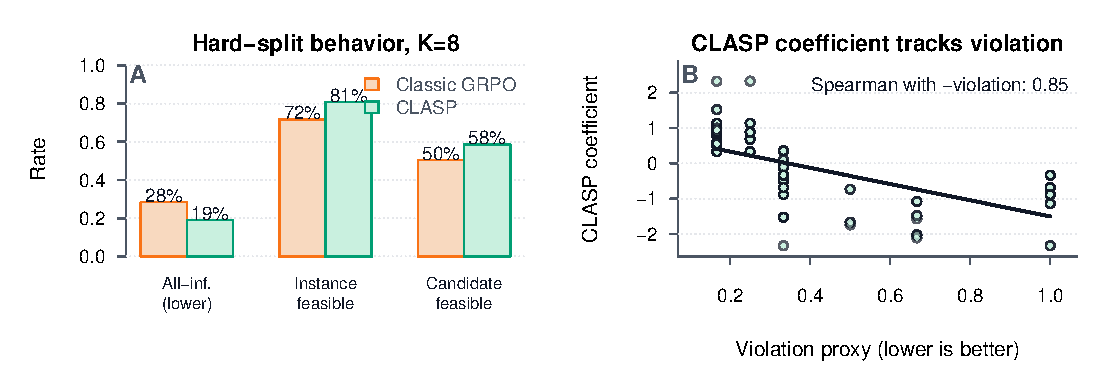
\includegraphics[width=0.95\linewidth]{figs/fig_inference_hard_group_main.pdf}
  \caption{\textbf{Inference hard-group diagnostic.} Left: on the hard split with \(K=8\) candidates per prompt, CLASP reduces all-infeasible groups and improves instance- and candidate-level feasibility relative to classic GRPO. Right: on all-infeasible groups with observable violation variation, the CLASP grouped advantage is negatively associated with the violation proxy, indicating that lower-violation candidates receive larger grouped advantages. The violation proxy is \(\max(0,1-\gamma)\), where \(\gamma\) is the logged \texttt{constraint\_fraction}.}
  \label{fig:hard_group_main}
\end{figure}

\subsection{CLASP-GRPO}
The current CLASP implementation is aligned with the deployment metric used in evaluation: best feasible solution in a group of \(K\) samples. Let \(q_i\) be a high-is-better objective score, \(v_i\geq 0\) the total violation, and \(z_i=\mathbf{1}[v_i=0]\) the feasibility flag. For a group \(G\), define the set utility
\begin{align}
U(G) =
\begin{cases}
\operatorname{smoothmax}_{i:z_i=1}(q_i), & \sum_i z_i>0,\\
-\lambda_G, & \sum_i z_i=0.
\end{cases}
\label{eq:bonutility}
\end{align}
The exact leave-one-out credit is the marginal
\begin{align}
\Delta_i^{\mathrm{LOO}} = U(G)-U(G\setminus\{i\}).
\label{eq:claspadv}
\end{align}
The canonical training path uses the implementation's dense-rank estimator rather than this expensive exact marginal for every update. In successful mixed groups, every feasible completion is ranked above every infeasible completion, while feasible completions receive tie-aware objective rank credit and infeasible completions receive lower-violation rank credit. The resulting credit is centered within the group. In an all-infeasible group, the estimator uses a robust, centered lower-violation rank surrogate, with recovery pressure scaled by \(1+\lambda_G\). Thus the implementation provides a signal for recovery even when the best-of-\(K\) set utility is flat before a feasible completion is observed.

The group multiplier \(\lambda_G\) is expanded from taskwise controller state and updated by projected signed-gap statistics at the configured update interval. These signed gaps are a controller signal, not the definition of the set utility. The canonical source configuration uses \(K=8\), dense-rank success credit, token-level importance sampling, no length penalty (\(\alpha=0\)), no inference repair, and the recorded canonical scale parameters. The exact behavior is implemented in \texttt{compute\_bon\_aligned\_advantages} and must be read together with the frozen source snapshot recorded in the paper manifest.

This definition is intentionally narrower than the historical manuscript's centered \((r,g)\) mixture. The current results must not be described using the old logistic mixing coefficient, centered primal/gap equation, adaptive controller claim, or historical all-infeasible recovery percentages unless their source receipts are independently recovered. The retained diagnostic figures are legacy artifacts until regenerated from current receipts.

\begin{figure}[!t]
  \centering
  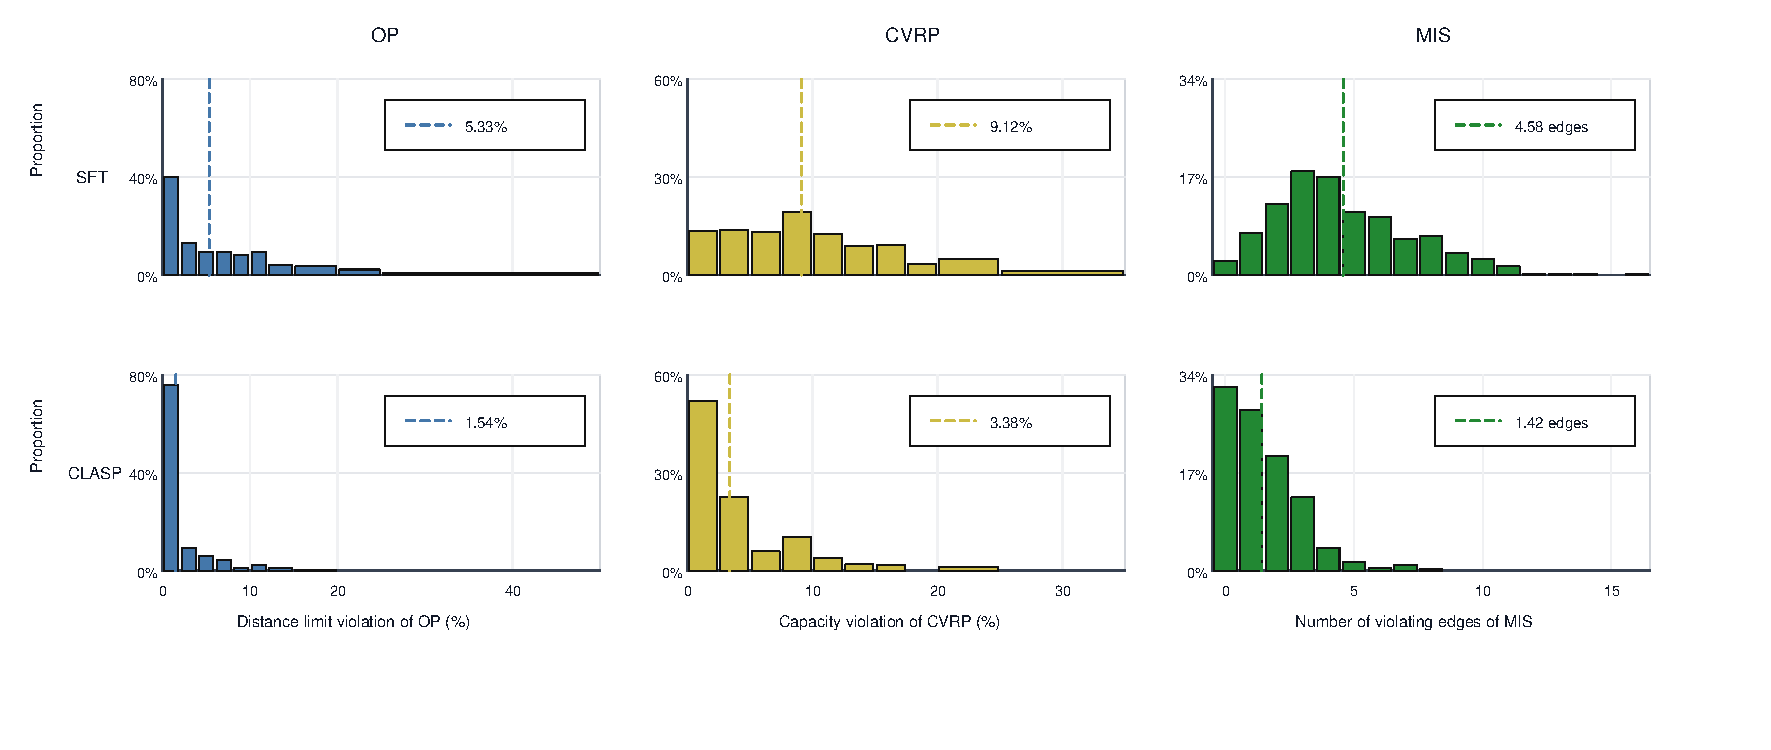
\includegraphics[width=0.82\linewidth]{figs/fig10_sft_clasp_high_delta_violation_histograms.pdf}
  \caption{Constraint-violation distributions for SFT and CLASP on high-violation prompts across tasks. The dashed line in each panel marks the mean policy statistic for that problem. Lower violation mass indicates better feasibility behavior.}
  \label{fig:sft_clasp_violation_hist}
\end{figure}

Our formal analysis focuses on a limited set of properties and is deferred to Appendix~\ref{app:formal}. There, we show that population-level feasibility aligns with the dense-cost constraints under mask completeness, that reference-sample terms cancel under group centering, that the grouped advantage remains non-degenerate in a specific all-infeasible regime, and that the projected signed-gap controller satisfies fixed-point sign conditions. These results provide theoretical support for the mechanism underlying CLASP, but they do not imply unbiasedness, convergence, or exact optimization guarantees for the practical training algorithm.

\begin{algorithm}[t]
\caption{One CLASP-GRPO training step.}
\label{alg:claspgrpo}
\small
\KwIn{Current policy \(\pi_\theta\), old policy \(\pi_{\mathrm{old}}\), taskwise controller weights \(\Lambda\), mixed-task prompt batch \(\{x_b,\tau_b\}_{b=1}^B\)}
\KwOut{Updated policy parameters and taskwise controller weights}
Sample a mixed-task batch and generate \(K\) completions per prompt from \(\pi_{\mathrm{old}}\)\;
Parse each completion and compute objective quality \(q_i\), dense costs \(\mathbf{c}_i^{(\tau)}\), masks \(\mathbf{m}_i^{(\tau)}\), exact violation \(v_i\), feasibility \(z_i\), and componentwise signed gaps \(h_{ij}^{(\tau)}\)\;
For each prompt group, form the best-of-\(K\) set utility and the dense-rank success or all-infeasible recovery credit described above\;
Center the selected credit within the group to obtain \(A_i^{\mathrm{CLASP}}\)\;
Apply the clipped sequence-level policy update using \(A_i^{\mathrm{CLASP}}\)\;
Every \(n_\lambda\) primal steps, update the taskwise controller weights using Eq.~\eqref{eq:claspdual}\;
Refresh each task's decoding budget from a rolling quantile of observed completion lengths\;
\end{algorithm}

\subsection{Task-Adaptive Completion Length}
The third component of CLASP is computational. Feasible outputs can differ dramatically in length across tasks: a TSP route is short, whereas a JSSP schedule can be much longer. A single global completion cap therefore mismatches compute allocation to task structure. For each task \(\tau\), CLASP maintains a rolling buffer of decoded lengths and periodically sets
\begin{align}
L_\tau \leftarrow \min\!\left\{L_{\max},\max\!\left\{L_{\min},Q_q(\mathrm{buf}_\tau)+32\right\}\right\},
\label{eq:adaptivelen}
\end{align}
where \(Q_q\) is the empirical \(q\)-quantile. Before the buffer is sufficiently populated, the implementation leaves the task budget at the global cap \(L_{\max}\). This mechanism does not change the optimization objective, but it changes how rollout budget is distributed across tasks and reduces unnecessary truncation or over-allocation.
Its role is mainly practical: it helps a single training loop allocate generation budget more sensibly across tasks with very different output lengths.

\subsection{Population Objective and Estimator Analysis}
The dense-cost construction induces a constrained multi-task objective that motivates, but does not exactly characterize, the practical algorithm. For each task \(\tau\), let \(x\sim\mathcal D_\tau\) denote a prompt and \(y\sim\pi_\theta(\cdot\mid x)\) a sampled completion. Define
\begin{align}
J_{\tau,x}(\theta)
&=
\mathbb{E}_{y\sim\pi_\theta(\cdot\mid x)}\bigl[r^{(\tau)}(x,y)\bigr],
\\
J_\tau(\theta)
&=
\mathbb{E}_{x\sim\mathcal D_\tau}\bigl[J_{\tau,x}(\theta)\bigr],
\end{align}
and the nonnegative thresholded-feasibility moments
\begin{align}
V_{\tau,j}(\theta)
=
\mathbb{E}_{x\sim\mathcal D_\tau,\,y\sim\pi_\theta(\cdot\mid x)}
\Bigl[m_j^{(\tau)}(x,y)\max\!\left\{0,c_j^{(\tau)}(x,y)-\epsilon_j^{(\tau)}\right\}\Bigr].
\label{eq:positiveconstraint}
\end{align}
Because the integrand is nonnegative, the feasible set is the equality set \(V_{\tau,j}(\theta)=0\) for all active task components, equivalently written as \(V_{\tau,j}(\theta)\le 0\). Under the mask-completeness assumption, this aligns the population constraints with thresholded feasibility rather than with cancellation in expectation.
If \(p_{\mathrm{task}}(\tau)\) denotes the effective task-sampling distribution of the mixed-task loader, the corresponding multi-task Lagrangian is
\begin{align}
\mathcal L(\theta,\Lambda)
=
\sum_{\tau\in\mathcal T} p_{\mathrm{task}}(\tau)
\left[
J_\tau(\theta) - \sum_{j=1}^{m_\tau} \lambda_j^{(\tau)} V_{\tau,j}(\theta)
\right].
\label{eq:multitasklagrangian}
\end{align}
This sign convention corresponds to a primal maximization problem with equivalent inequalities \(V_{\tau,j}(\theta)\le 0\): larger \(\lambda_j^{(\tau)}\) penalizes positive violation in the inner maximization. CLASP should therefore be read as a grouped stochastic method motivated by this reference objective, not as an algorithm proved to optimize Eq.~\eqref{eq:multitasklagrangian} exactly. Because the grouped advantage depends on prompt-local feasibility through \(\alpha_G\) and on within-group normalization through \((\bar r_G,\bar g_G,\sigma_r^G,\sigma_g^G)\), the finite-\(K\) estimator does not collapse to a single centered scalarization with fixed global weights. The controller also updates from signed masked gaps because they provide a stable directional signal even when many samples lie strictly inside the feasible region.

Define the signed surrogate constraint moments
\begin{align}
G_{\tau,j}(\theta)
=
\mathbb{E}_{x\sim\mathcal D_\tau,\,y\sim\pi_\theta(\cdot\mid x)}
\Bigl[m_j^{(\tau)}(x,y)\bigl(c_j^{(\tau)}(x,y)-\epsilon_j^{(\tau)}\bigr)\Bigr].
\label{eq:signedconstraint}
\end{align}
The projected update in Eq.~\eqref{eq:claspdual} is a controller defined on minibatch estimates of \(G_{\tau,j}\). Proposition~\ref{prop:controller-fixed-point} characterizes the fixed points of that controller rather than exact optimization of Eq.~\eqref{eq:multitasklagrangian}. In particular, zeros of \(G_{\tau,j}\) do not exclude cancellation between positive and negative deviations around \(\epsilon_j^{(\tau)}\).

The exact positive violation score can be written as
\begin{align}
v^{(\tau)}(x,y)
=
\sum_{j=1}^{m_\tau} m_j^{(\tau)}(x,y)
\max\!\left\{0,c_j^{(\tau)}(x,y)-\epsilon_j^{(\tau)}\right\}.
\end{align}
Then thresholded feasibility is equivalent to \(v^{(\tau)}(x,y)=0\). Appendix~\ref{app:formal} collects the formal statements: the population constraints align with thresholded feasibility under mask completeness, the grouped advantage is well-defined, reference-sample constants cancel under group centering, the grouped advantage remains non-trivial in a specific all-infeasible constant-primal regime, and the projected controller satisfies complementary-sign fixed-point conditions. The regularity assumptions needed for these results are deferred to the appendix.
\section{Experiments}
\label{sec:experiments}
We evaluate the current implementation under a frozen matched development protocol and keep decoder tuning on a disjoint development slice. The canonical reproduction uses four A100 GPUs for training and one A100 GPU per evaluation job; it is not an exact historical-source reproduction. The standalone vanilla GRPO row in the legacy manuscript is not promoted to the current comparison without a validated receipt. Unless stated otherwise, the five-task data originate from \citet{jiang2025endtoendco}; exact slices, checkpoint lineage, decoding parameters, and caveats are recorded in the paper manifest.

Our benchmark covers five tasks: TSP, OP, CVRP, MIS, and JSSP. Unless noted otherwise, learned methods share the same base model family, prompt template, tokenizer, task mixture, and two-stage pipeline of mixed-task SFT followed by RL. We defer full training and data details to Appendix~\ref{app:expdetails}.

At evaluation time, we recompute every objective value from the parsed discrete solution rather than from the model's self-reported score. We report candidate feasibility rate, instance feasibility rate, and mean/median best-feasible reference gap. Mean and median gaps are conditional on instances for which the method finds at least one feasible candidate; infeasible instances are captured by the feasibility columns and by Success@\(k\) rates. Because conditional gaps can favor methods that solve only easier instances, we do not use the gap column alone to rank methods when feasibility differs substantially; we interpret each gap together with its corresponding feasibility rate and use Success@\(k\) as an all-instance threshold metric. These metrics separate the ability to find any feasible solution from the ability to find a good one; gap definitions, tie-breaking rules, candidate budgets, and dataset diagnostics are given in Appendix~\ref{app:expdetails}.

\begin{table*}[t]
\caption{Results on the five tasks shared with \citet{jiang2025endtoendco}: TSP, OP, CVRP, MIS, and JSSP. All results are on our OOD held-out set. Higher feasibility (fea.) and lower reference-value gap (opt.) are better, where the reference value is solver generated near optimal solution. The opt. columns are conditional on instances with at least one feasible candidate and should be read together with feasibility; infeasible instances receive no artificial gap value and count as failures in Success@\(k\) metrics. Under \textbf{This work}, BoN means best-of-\(N\) decoding with \(N=8\), and 2500k/250k denote the base SFT dataset size before RL (500{,}000/50{,}000 examples per task).}
\label{tab:main}
\centering
\scriptsize
\resizebox{\textwidth}{!}{%
\begin{tabular}{lcccccccccc}
\toprule
Method & \multicolumn{2}{c}{TSP} & \multicolumn{2}{c}{OP} & \multicolumn{2}{c}{CVRP} & \multicolumn{2}{c}{MIS} & \multicolumn{2}{c}{JSSP} \\
\cmidrule(lr){2-3}\cmidrule(lr){4-5}\cmidrule(lr){6-7}\cmidrule(lr){8-9}\cmidrule(lr){10-11}
 & fea. & opt. & fea. & opt. & fea. & opt. & fea. & opt. & fea. & opt. \\
\midrule
\multicolumn{11}{l}{\textbf{General-purpose Language Models}} \\
GPT-4o & 39\% & 33.79\% $\pm$ 16.6 & 59\% & 55.19\% $\pm$ 15.7 & 15\% & 76.62\% $\pm$ 7.9 & 8\% & 11.70\% $\pm$ 11.8 & 7\% & 97.85\% $\pm$ 23.7 \\
GPT-4o-mini & 28\% & 53.38\% $\pm$ 21.5 & 80\% & 70.70\% $\pm$ 10.3 & 3\% & 68.10\% $\pm$ 10.5 & 1\% & 0.00\% $\pm$ 0 & 8\% & 212\% $\pm$ 121 \\
Claude-Sonnet & 66\% & 24.53\% $\pm$ 10.7 & 49\% & 34.62\% $\pm$ 14.1 & 30\% & 38.34\% $\pm$ 15.9 & 13\% & 12.51\% $\pm$ 12.5 & 10\% & 90.00\% $\pm$ 21.6 \\
Claude-Haiku & 45\% & 38.60\% $\pm$ 16.9 & 26\% & 51.26\% $\pm$ 14.9 & 4\% & 61.48\% $\pm$ 12.1 & 2\% & 23.33\% $\pm$ 6.7 & 9\% & 95.51\% $\pm$ 22.2 \\
DeepSeek-V3 & 73\% & 35.75\% $\pm$ 15.4 & 50\% & 46.10\% $\pm$ 13.4 & 21\% & 58.22\% $\pm$ 26.8 & 5\% & 12.05\% $\pm$ 12.9 & 52\% & 103.19\% $\pm$ 26.9 \\
Llama3.3-70B & 50\% & 69.08\% $\pm$ 31.4 & 27\% & 48.98\% $\pm$ 14.6 & 31\% & 97.31\% $\pm$ 69.3 & 8\% & 37.12\% $\pm$ 29.5 & 29\% & 105.01\% $\pm$ 24.5 \\
Qwen2.5-72B & 20\% & 36.89\% $\pm$ 34.6 & 32\% & 49.36\% $\pm$ 16.6 & 61\% & 180.91\% $\pm$ 105 & 14\% & 29.56\% $\pm$ 16.2 & 53\% & 103.90\% $\pm$ 61.7 \\
\addlinespace[2pt]
\multicolumn{11}{l}{\textbf{Reasoning Models}} \\
GPT-o3-mini & 91\% & 306\% $\pm$ 258 & 8\% & 43.93\% $\pm$ 11.5 & 50\% & 139\% $\pm$ 39.7 & 66\% & 9.23\% $\pm$ 8.4 & 20\% & 77.86\% $\pm$ 37.8 \\
GPT-o1 & 54\% & 276\% $\pm$ 242 & 31\% & 40.90\% $\pm$ 16.3 & 24\% & 154\% $\pm$ 117 & 82\% & 8.03\% $\pm$ 12.9 & 29\% & 81.90\% $\pm$ 29.6 \\
DeepSeek-R1 & 48\% & 70.99\% $\pm$ 23.1 & 60\% & 40.54\% $\pm$ 13.7 & 26\% & 30.46\% $\pm$ 18.1 & 41\% & 1.60\% $\pm$ 3.6 & 5\% & 26.29\% $\pm$ 8.5 \\
\addlinespace[2pt]
\multicolumn{11}{l}{\textbf{Prompt Strategies}} \\
OPRO & 83\% & 35.98\% $\pm$ 3.6 & 85\% & 53.96\% $\pm$ 14.3 & 21\% & 37.03\% $\pm$ 18.3 & 7\% & 5.95\% $\pm$ 7.3 & 65\% & 83.35\% $\pm$ 25.5 \\
LMEA & 77\% & 265\% $\pm$ 131 & 48\% & 66.18\% $\pm$ 10.5 & 24\% & 61.24\% $\pm$ 19.0 & 5\% & 25.0\% $\pm$ 14.2 & 44\% & 83.19\% $\pm$ 23.9 \\
PHP & 84\% & 33.84\% $\pm$ 14.6 & 43\% & 36.08\% $\pm$ 15.1 & 33\% & 58.11\% $\pm$ 26.4 & 5\% & 11.67\% $\pm$ 9.1 & 56\% & 104.04\% $\pm$ 29.2 \\
SGE & 98\% & 29.66\% $\pm$ 43.3 & 93\% & 24.49\% $\pm$ 38.4 & 84\% & 36.14\% $\pm$ 59.2 & 92\% & 3.62\% $\pm$ 7.6 & 87\% & 38.58\% $\pm$ 49.2 \\
\addlinespace[2pt]
\multicolumn{11}{l}{\textbf{Base paper (Jiang et al.)}} \\
Jiang et al. SFT 2500k & 89\% & 2.30\% $\pm$ 1.9 & 54\% & 2.32\% $\pm$ 2.6 & 59\% & 6.02\% $\pm$ 3.9 & 80\% & 1.71\% $\pm$ 3.9 & 100\% & 11.01\% $\pm$ 7.9 \\
Base SFT+classicGRPO 2500k & 91\% & 2.32\% $\pm$ 2.2 & 92\% & 4.25\% $\pm$ 2.9 & 80\% & 8.27\% $\pm$ 5.6 & 83\% & 1.34\% $\pm$ 3.3 & 100\% & 10.94\% $\pm$ 7.3 \\
Jiang et al. SFT+RL+BoN 2500k & 100\% & 1.07\% $\pm$ 0.9 & 100\% & 1.85\% $\pm$ 1.7 & 100\% & 4.53\% $\pm$ 3.5 & 94\% & 1.04\% $\pm$ 3.4 & 100\% & 8.20\% $\pm$ 6.3 \\
\addlinespace[2pt]
\multicolumn{11}{l}{\textbf{This work}} \\
SFT+BoN 250k & 99.3\% & 2.26\% $\pm$ 1.86 & 95.7\% & 1.54\% $\pm$ 2.59 & 61.3\% & 5.32\% $\pm$ 4.19 & 74.0\% & 1.45\% $\pm$ 3.71 & 90.3\% & 9.08\% $\pm$ 7.13 \\
Vanilla GRPO+BoN 250k & 100.0\% & 2.18\% $\pm$ 1.54 & 99.7\% & 1.42\% $\pm$ 1.73 & 97.0\% & 8.04\% $\pm$ 4.65 & 87.3\% & 4.19\% $\pm$ 7.15 & 59.0\% & 6.19\% $\pm$ 5.01 \\
Dual-primal GRPO+BoN 250k & 100.0\% & 2.10\% $\pm$ 1.54 & 95.3\% & 1.22\% $\pm$ 1.69 & 92.0\% & 6.01\% $\pm$ 3.99 & 88.3\% & 4.37\% $\pm$ 7.50 & 90.3\% & 8.49\% $\pm$ 6.19 \\
CLASP+BoN (ours) 250k & \textbf{100\%} & \textbf{1.01\% $\pm$ 0.91} & 98\% & \textbf{1.18\% $\pm$ 1.38} & \textbf{100\%} & \textbf{4.18\% $\pm$ 1.97} & \textbf{96\%} & \textbf{1.04\% $\pm$ 3.71} & \textbf{100\%} & \textbf{8.19\% $\pm$ 6.13} \\
\bottomrule
\end{tabular}%
}
\end{table*}

\begin{table}[!t]
\centering
\caption{Comparison with problem-specific solvers (LKH for TSP, EA4OP for OP, HGS for CVRP, and Gurobi for MIS and JSSP), Gurobi, and CLASP. Results are reported as optimality gap(time), and ``-'' denotes an infeasible solution. The CLASP row uses the same best-of-8 setting as Table~\ref{tab:main}; its time includes decoding, parsing, rescoring, and feasible-candidate selection.}
\label{tab:sota_solver_comparison}
\tiny
\resizebox{0.78\linewidth}{!}{%
\begin{tabular}{lccccc}
\toprule
Method & TSP & OP & CVRP & MIS & JSSP \\
\midrule
SOTA method & 0.00\%(0.3) & 1.60\%(0.3) & -0.19\%(1.2) & 0.00\%(1.0) & 2.45\%(10.0) \\
Gurobi (1s) & 5.76\%(1.0) & 49.42\%(1.0) & -- & 2.28\%(1.0) & 41.34\%(1.0) \\
Gurobi (10s) & 1.82\%(10.0) & 21.96\%(10.0) & 35.09\%(10.0) & 0.46\%(10.0) & 2.45\%(10.0) \\
CLASP & 1.01\%(7.34) & 1.18\%(5.28) & 4.18\%(7.96) & 1.04\%(3.28) & 8.19\%(11.72) \\
\bottomrule
\end{tabular}
}
\end{table}





\FloatBarrier

The broader reference comparison helps separate aggregate gains from distributional ones. Table~\ref{tab:scale_subset} provides a size-stratified diagnostic for the five-task subset. For the local learned-method rows, the scale bins are computed from the same full-300 logs as Table~\ref{tab:main}; because opt. gaps are conditional on feasibility, aggregate gaps are recovered by feasible-count weighting over bins rather than by an unweighted average. The small/medium/large grouping follows the benchmark scale convention. For scheduling problems with jobs and machines, such as PFSP and JSSP, scale is defined by the job--machine grid: small covers \(5\times5\) to \(10\times10\), medium covers \(10\times10\) to \(15\times15\), and large covers \(15\times15\) to \(20\times20\). For all other graph, routing, and subset-selection problems, such as TSP, OP, CVRP, MIS, and MVC, scale is defined by the number of nodes: small covers \(10\)--\(30\) nodes, medium covers \(40\)--\(60\) nodes, and large covers \(70\)--\(100\) nodes. We move the matched Taillard-format JSSP comparison to Appendix~\ref{app:additional_results}.

\begin{table*}[t]
\caption{Results by problem scale on the five-task subset shared with \citet{jiang2025endtoendco}, evaluated on our OOD held-out set. Scheduling scales are defined by job--machine grids: small \(5\times5\)--\(10\times10\), medium \(10\times10\)--\(15\times15\), and large \(15\times15\)--\(20\times20\); non-scheduling scales are defined by node counts: small \(10\)--\(30\), medium \(40\)--\(60\), and large \(70\)--\(100\). Gap is the mean best-feasible reference gap within each scale bin, while Success@\(k\) is the percentage of all instances in the bin with a feasible candidate within \(k\%\) of the reference. Lower gap and higher Success@\(k\) are better; aggregate rows and scale-stratified rows should only be compared when they are generated from the same evaluation protocol and candidate set.}
\label{tab:scale_subset}
\centering
\scriptsize
\resizebox{\textwidth}{!}{%
\begin{tabular}{lcccccccccccc}
\toprule
Method & \multicolumn{4}{c}{Small instances} & \multicolumn{4}{c}{Medium instances} & \multicolumn{4}{c}{Large instances} \\
\cmidrule(lr){2-5}\cmidrule(lr){6-9}\cmidrule(lr){10-13}
 & Gap & Success@1 & Success@5 & Success@10 & Gap & Success@1 & Success@5 & Success@10 & Gap & Success@1 & Success@5 & Success@10 \\
\midrule
\multicolumn{13}{l}{\textbf{TSP}} \\
OR-Tools & 0.82\% & 76\% & 96\% & 99\% & 2.59\% & 28\% & 86\% & 99\% & 3.59\% & 12\% & 80\% & 99\% \\
NN & 19.36\% & 3\% & 5\% & 19\% & 24.13\% & 0\% & 0\% & 1\% & 26.19\% & 0\% & 0\% & 2\% \\
FI & 2.27\% & 51\% & 82\% & 96\% & 4.41\% & 8\% & 64\% & 95\% & 4.86\% & 2\% & 53\% & 99\% \\
ACO & 1.98\% & 48\% & 88\% & 100\% & 17.98\% & 0\% & 1\% & 6\% & 36.69\% & 0\% & 0\% & 0\% \\
Jiang et al. & 0.14\% & 96\% & 100\% & 100\% & 0.70\% & 74\% & 100\% & 100\% & 1.34\% & 44\% & 100\% & 100\% \\
Dual-primal GRPO & 1.32\% & 55\% & 98\% & 100\% & 2.23\% & 18\% & 93\% & 100\% & 2.75\% & 10\% & 95\% & 100\% \\
CLASP & 0.62\% & 52\% & 100\% & 100\% & 1.09\% & 25\% & 95\% & 100\% & 1.32\% & 6\% & 97\% & 100\% \\
\addlinespace[2pt]
\multicolumn{13}{l}{\textbf{OP}} \\
Greedy & 16.06\% & 4\% & 8\% & 25\% & 18.91\% & 0\% & 0\% & 5\% & 20.30\% & 0\% & 0\% & 3\% \\
GI & 9.07\% & 20\% & 37\% & 63\% & 11.91\% & 0\% & 12\% & 51\% & 13.63\% & 0\% & 7\% & 32\% \\
Tsili & 3.85\% & 21\% & 68\% & 96\% & 9.54\% & 0\% & 2\% & 55\% & 13.80\% & 0\% & 0\% & 8\% \\
ACO & 3.49\% & 30\% & 76\% & 94\% & 6.24\% & 1\% & 35\% & 89\% & 7.95\% & 0\% & 15\% & 74\% \\
Jiang et al. & 1.47\% & 54\% & 95\% & 99\% & 2.04\% & 26\% & 96\% & 100\% & 2.10\% & 27\% & 96\% & 99\% \\
Dual-primal GRPO & 0.70\% & 79\% & 91\% & 94\% & 1.13\% & 57\% & 93\% & 96\% & 1.83\% & 32\% & 92\% & 95\% \\
CLASP & 0.55\% & 79\% & 94\% & 95\% & 1.23\% & 57\% & 95\% & 96\% & 1.75\% & 37\% & 90\% & 93\% \\
\addlinespace[2pt]
\multicolumn{13}{l}{\textbf{CVRP}} \\
OR-Tools & 3.60\% & 45\% & 69\% & 93\% & 7.87\% & 3\% & 24\% & 72\% & 8.84\% & 0\% & 15\% & 71\% \\
Sweep & 18.36\% & 8\% & 18\% & 32\% & 20.59\% & 0\% & 1\% & 8\% & 22.07\% & 0\% & 0\% & 3\% \\
PS & 3.95\% & 24\% & 72\% & 93\% & 5.67\% & 2\% & 50\% & 89\% & 6.12\% & 0\% & 41\% & 89\% \\
ACO & 2.52\% & 44\% & 81\% & 96\% & 17.07\% & 0\% & 2\% & 14\% & 29.49\% & 0\% & 0\% & 0\% \\
Jiang et al. & 1.70\% & 52\% & 90\% & 97\% & 4.57\% & 8\% & 59\% & 98\% & 7.24\% & 1\% & 19\% & 84\% \\
Dual-primal GRPO & 3.40\% & 27\% & 70\% & 95\% & 6.19\% & 2\% & 37\% & 80\% & 9.03\% & 0\% & 6\% & 48\% \\
CLASP & 2.57\% & 29\% & 66\% & 92\% & 3.99\% & 2\% & 44\% & 85\% & 5.98\% & 0\% & 10\% & 59\% \\
\addlinespace[2pt]
\multicolumn{13}{l}{\textbf{MIS}} \\
Degree & 5.89\% & 57\% & 57\% & 67\% & 7.52\% & 32\% & 42\% & 64\% & 9.61\% & 20\% & 33\% & 59\% \\
Greedy & 2.56\% & 84\% & 84\% & 86\% & 2.79\% & 67\% & 71\% & 90\% & 3.36\% & 53\% & 60\% & 83\% \\
Jiang et al. & 0.38\% & 97\% & 98\% & 98\% & 1.05\% & 86\% & 87\% & 94\% & 2.29\% & 47\% & 57\% & 65\% \\
Dual-primal GRPO & 1.91\% & 84\% & 84\% & 89\% & 5.18\% & 54\% & 62\% & 77\% & 6.87\% & 31\% & 42\% & 49\% \\
CLASP & 0.44\% & 83\% & 83\% & 89\% & 1.16\% & 53\% & 61\% & 78\% & 1.52\% & 31\% & 45\% & 50\% \\
\addlinespace[2pt]
\multicolumn{13}{l}{\textbf{JSSP}} \\
SPT & 19.58\% & 2\% & 4\% & 17\% & 25.32\% & 0\% & 0\% & 1\% & 27.35\% & 0\% & 0\% & 0\% \\
FIFO & 24.38\% & 2\% & 4\% & 12\% & 32.97\% & 0\% & 0\% & 1\% & 39.00\% & 0\% & 0\% & 0\% \\
ATC & 20.71\% & 0\% & 12\% & 15\% & 24.30\% & 0\% & 0\% & 1\% & 27.99\% & 0\% & 0\% & 0\% \\
Jiang et al. & 2.86\% & 32\% & 79\% & 98\% & 9.56\% & 0\% & 8\% & 60\% & 16.25\% & 0\% & 0\% & 4\% \\
Dual-primal GRPO & 4.44\% & 29\% & 61\% & 92\% & 7.88\% & 11\% & 34\% & 65\% & 15.05\% & 0\% & 0\% & 9\% \\
CLASP & 4.09\% & 27\% & 58\% & 87\% & 6.93\% & 5\% & 34\% & 69\% & 13.55\% & 0\% & 0\% & 12\% \\
\bottomrule
\end{tabular}%
}
\end{table*}

\FloatBarrier


\section{Conclusion}
For LLM-based combinatorial optimization, the central challenge is not only to improve objective quality, but to do so without losing feasibility. Our results show that this requires a stronger within-group learning signal than centered scalar reward alone. CLASP-GRPO addresses this issue with an adaptive centered grouped advantage, a feasibility-conditional signed-gap controller, and task-adaptive decoding budgets. Across five combinatorial optimization tasks, it consistently improves feasibility-preserving generation over centered GRPO baselines and remains competitive with the closest prior LLM-based CO system under matched compute and candidate budgets. This comparison is especially notable because our SFT stage uses 10 times less supervised data than the reproduced Jiang et al. setting, allowing us to test how well CLASP learns under substantially more data-constrained supervision. More broadly, the results indicate that grouped reinforcement learning for constrained generation becomes substantially more effective when prompt-local comparisons are structured around feasibility and quality jointly, rather than around a single centered reward. CLASP is therefore a practical and lightweight method for improving feasibility-aware LLM optimization, though it is not a replacement for specialized solvers. 

\FloatBarrier
\clearpage
\bibliographystyle{plainnat}
\bibliography{references}

\clearpage
\appendix

\section{Data Pipeline and SFT Details}
\label{app:dataflow}
Both training stages operate on a unified instance representation so that cross-task differences arise from the tasks themselves rather than from incompatible preprocessing. Each raw example is mapped into the common fields \texttt{instruction}, \texttt{input}, \texttt{output}, and \texttt{instance\_json}. Duplicates are removed within each split, and task sizes are capped when needed to control mixture balance. If a task provides separate evaluation files, we eliminate exact within-task train/eval overlap. Otherwise, evaluation uses a held-out partition carved from the task's available training data, while any reserved evaluation files remain untouched until post-training comparison.

For the shared five-task comparison with \citet{jiang2025endtoendco}, we use the same train and evaluation datasets on the overlapping tasks, but reduce the supervised stage to 50{,}000 SFT examples per task instead of the 500{,}000-per-task SFT setting used in the reproduced Jiang et al. configuration. The reference solutions in these datasets are solver-generated rather than model-generated. Specifically, \textbf{TSP} reference solutions are generated with the Lin--Kernighan--Helsgaun (LKH-3) solver and serve as optimal or best-known references for the 10--100 node instances used here; \textbf{OP} reference solutions are generated using the EA4OP genetic-algorithm-based solver; \textbf{CVRP} reference solutions are near-optimal solutions produced by LKH-3; \textbf{MIS} reference solutions are optimal solutions obtained with the Gurobi exact solver; and \textbf{JSSP} reference solutions are near-optimal solutions computed with the CP-SAT solver from Google OR-Tools using a 300-second time limit.

For SFT, each example is mapped to
\begin{align}
\texttt{prompt}_i &= \mathrm{Prompt}(\texttt{instruction}_i, \texttt{input}_i), \\
\texttt{completion}_i &= \texttt{output}_i \oplus \texttt{eos}, \\
\texttt{text}_i &= \texttt{prompt}_i \oplus \texttt{completion}_i.
\end{align}
For supervision, we align loss with the generated answer whenever tokenization preserves the prompt as an exact prefix of the full sequence; in those cases, optimization is performed on the completion tokens alone. If that alignment is broken by tokenization, we instead optimize over the full prompt--completion sequence to avoid masking errors. In multi-task runs, batches are constructed to maintain task diversity whenever more than one task is active, and the same mixture policy is retained during GRPO so that differences between stages are attributable to the learning objective rather than to a shift in task composition.

\section{Controller, Claims, and Experimental Details}
\label{app:controller}
\subsection{Reward and Controller Details}
The primal score combines a small structure reward with an objective reward. For every task,
\begin{align}
s_i
&= \frac{1}{3}\Bigl(
\mathbf{1}[\text{required block exists}] \notag\\
&\qquad + \mathbf{1}[\text{parser returns a non-empty structure}] \notag\\
&\qquad + \mathbf{1}[\text{declared objective/makespan exists}]
\Bigr),
\end{align}
so \(s_i \in [0,1]\). This term rewards parser-compatible formatting rather than feasibility itself.

Objective quality is measured relative to the reference output in the RL data. Let \(\delta_i\) denote the signed relative gap, positive when the candidate is worse than the reference and negative when it is better:
\begin{align}
\delta_i =
\begin{cases}
\dfrac{\mathrm{pred}_i - \mathrm{ref}_i}{\mathrm{ref}_i}, & \text{minimization}, \\
\dfrac{\mathrm{ref}_i - \mathrm{pred}_i}{\mathrm{ref}_i}, & \text{maximization}.
\end{cases}
\end{align}
We then map this gap to
\begin{align}
\psi(\delta_i) =
\begin{cases}
\exp(-3 \delta_i), & \delta_i \ge 0, \\
1 + 0.5 \tanh(-2 \delta_i), & \delta_i < 0,
\end{cases}
\end{align}
and add a declaration-match bonus \(a_i \in \{0,1\}\) when the model's stated objective agrees with the value recomputed from the parsed structure. The ungated objective reward is
\begin{align}
\tilde{o}_i = 2 \left(0.9\, \psi(\delta_i) + 0.1\, a_i \right).
\end{align}
In the empirical study, we set \(w_o=1.0\) and \(w_s=0.3\) in \(r_i=w_o o_i+w_s s_i\).

For the clipped objective used in training, we use a \emph{length-normalized sequence surrogate ratio}. If \(T_i\) denotes the generated length,
\begin{align}
\rho_i(\theta) =
\exp\left(
\frac{1}{T_i}
\sum_{t=1}^{T_i}
\left[
\log \pi_\theta(y_{i,t} \mid x_i, y_{i,<t})
-
\log \pi_{\mathrm{old}}(y_{i,t} \mid x_i, y_{i,<t})
\right]
\right).
\label{eq:seqratio}
\end{align}
This quantity is the exponential of the average token-level log-likelihood ratio, equivalently the geometric mean of tokenwise likelihood ratios over the sampled sequence. It is therefore \emph{not} the exact sequence importance ratio \(\pi_\theta(y_i\mid x_i)/\pi_{\mathrm{old}}(y_i\mid x_i)\); rather, it is a bounded-scale surrogate used for numerical stability across outputs of different lengths. CLASP and Dual-primal GRPO use this surrogate and disable additional reward scaling. The vanilla GRPO row in Table~\ref{tab:main} follows the standard trainer objective, so it should be interpreted as a conventional system-level baseline; isolating the surrogate alone would require an additional sequence-surrogate vanilla GRPO ablation. Accordingly, the clipped objective below should be read as the practical training surrogate used in our constrained variants, not as a quantity inheriting the standard importance-sampling interpretation or PPO monotonic-improvement guarantees.
The clipped surrogate term is
\begin{align}
\ell_i(\theta) =
-\min\left(
\rho_i(\theta) A_i^{\mathrm{CLASP}},\;
\mathrm{clip}\!\left(\rho_i(\theta), 1-\epsilon_{\mathrm{low}}, 1+\epsilon_{\mathrm{high}}\right) A_i^{\mathrm{CLASP}}
\right),
\label{eq:clipsurrogate}
\end{align}
optionally with a KL regularizer of weight \(\kappa_{\mathrm{KL}}\).

We use \emph{Dual-primal GRPO} as the canonical name for the constrained GRPO baseline. It shares the same SFT initialization, prompt groups, dense cost components, length-normalized sequence ratio, and clipped surrogate family as CLASP, but it does not use the adaptive centered primal-gap grouped advantage in Eq.~\eqref{eq:claspadv}. Its sample advantage is
\begin{align}
A_i^{\mathrm{DP}}
=
\bigl(r_i-\bar r_G\bigr)
-
\sum_{j=1}^{m_\tau}\lambda_j^{(\tau)} h_{ij}^{(\tau)},
\label{eq:dualprimalbaseline}
\end{align}
with \(h_{ij}^{(\tau)}\) denoting the signed masked gap introduced above; the clipped surrogate above is then evaluated with \(A_i^{\mathrm{DP}}\) in place of \(A_i^{\mathrm{CLASP}}\). Thus the baseline centers only the primal reward within the prompt group and adds an uncentered controller-weighted signed-gap term, whereas CLASP centers both primal and controller-weighted positive-gap comparisons inside the adaptive grouped advantage.

Each task maintains its own controller \(\boldsymbol{\lambda}^{(\tau)}\). It acts as a practical weighting mechanism for feasibility pressure rather than exact dual ascent for the population Lagrangian. Under the sign convention of Eq.~\eqref{eq:multitasklagrangian}, the update is a projected signed-gap controller. Because minibatches are mixed-task but controllers are task-specific, the controller statistics are computed separately for each task. Let \(\mathcal B_t^{(\tau)}\) be the completions in the current controller window whose task is \(\tau\), and let \(N_t^{(\tau)}=|\mathcal B_t^{(\tau)}|\). Every \(n_\lambda\) primal steps, the task-local masked batch statistics are aggregated as
\begin{align}
\hat h_{t,j}^{(\tau)}
&=
\frac{1}{N_t^{(\tau)}} \sum_{i\in\mathcal B_t^{(\tau)}}
m_{ij}^{(\tau)} \bigl(c_{ij}^{(\tau)}-\epsilon_j^{(\tau)}\bigr), \\
\bar f_t^{(\tau)}
&=
\frac{1}{N_t^{(\tau)}} \sum_{i\in\mathcal B_t^{(\tau)}} \mathbf{1}[v_i = 0].
\end{align}
The controller then uses the feasibility-conditional step size
\begin{align}
\eta_\lambda^{(t,\tau)} = \eta_0 \sqrt{\frac{1-\bar f_t^{(\tau)}+\varepsilon}{\bar f_t^{(\tau)}+\varepsilon}}
\end{align}
and updates
\begin{align}
\lambda_{t+1,j}^{(\tau)}
=
\Pi_{[0,\lambda_{\max}]}
\left(
\lambda_{t,j}^{(\tau)} + \eta_\lambda^{(t,\tau)} \hat h_{t,j}^{(\tau)}
\right).
\label{eq:claspdual}
\end{align}
This rule reacts to the \emph{current} policy rather than to an exponential moving average of past violations. The projection keeps the controller in a compact domain and the shared step size couples controller aggressiveness to the observed feasibility regime. As in the main text, this appendix-level description is intentionally algorithmic: it specifies the mechanism used in practice, not a general convergence guarantee for the overall non-convex training dynamics.
For zero-tolerance components, the clipped costs have no negative interior margin and the corresponding controller weight can only increase or remain fixed, whereas positive-tolerance components can yield negative signed gaps and therefore allow the projected controller weight to decay.

CLASP also maintains a task-adaptive completion budget. For each task \(\tau\), a rolling window of recent decoded lengths is updated online; every \(R\) optimizer steps, the generation cap is reset to the clipped empirical quantile in Eq.~\eqref{eq:adaptivelen}. This leaves the reward definition unchanged, but it changes the effective compute allocation across tasks during RL.

\section{Claim Map and Experimental Setup}
\label{app:claimmap}
\begin{table}[t]
\caption{Evaluation questions and corresponding measurements. The table maps each empirical claim to the evidence reported in this manuscript, rather than to a complete possible ablation suite.}
\centering
\small
\begin{tabular}{p{0.33\linewidth}p{0.56\linewidth}}
\toprule
Claim & Evidence reported in this paper \\
\midrule
CLASP-GRPO improves feasibility & Table~\ref{tab:main} reports feasibility and conditional reference gaps for SFT+BoN, vanilla GRPO+BoN, Dual-primal GRPO+BoN, CLASP+BoN, and the Jiang et al. reference rows; Tables~\ref{tab:sota_solver_comparison}, \ref{tab:scale_subset}, \ref{tab:performance_comparison}, and \ref{tab:solving_time} add solver, scale-stratified, aggregate, and runtime context. \\
CLASP-GRPO improves best feasible quality & Table~\ref{tab:main} reports mean best-feasible reference gaps with dispersion for BoN=8, separately from feasibility; Table~\ref{tab:scale_subset} reports conditional gap and Success@\(1/5/10\) by size bin; Tables~\ref{tab:ta_subset} and \ref{tab:tsplib_gap_comparison_clasp} provide targeted Taillard JSSP and TSPLIB comparisons, including the reported TSPLIB BoN=8/64 distinction. \\
The proposed mechanism explains the gains & Mechanism evidence consists of the main hard-group diagnostic in Figure~\ref{fig:hard_group_main}, the training-variant comparison in Appendix Figure~\ref{fig:ablation_feasibility_bar}, the SFT-vs-CLASP violation distributions in Figure~\ref{fig:sft_clasp_violation_hist}, the appendix all-infeasible-group diagnostics in Figures~\ref{fig:all_infeasible_frequency} and \ref{fig:inference_hard_group_recovery}, the mechanism dashboard in Figure~\ref{fig:mechanism_dashboard}, and the training-dynamics curves in Figure~\ref{fig:curves}. Tables~\ref{tab:data}, \ref{tab:diagnostics}, and \ref{tab:rl_hparams}, together with Appendix~\ref{app:costs}, define the data, sequence-pressure diagnostics, training settings, adaptive length mechanism, dense costs, infeasible-sample credit, feasibility rule, and controller parameters used by those diagnostics. \\
\bottomrule
\end{tabular}
\end{table}

\section{Benchmark and Configuration Details}
\label{app:expdetails}
\begin{table*}[t]
\caption{Benchmark suite used in this paper. The table summarizes the tasks, data volumes, and output schemas used in the supported experimental setup. Reported SFT train-set sizes correspond to the subsets actually used in the experiments, before within-split deduplication and train/validation partitioning; each task uses 50{,}000 supervised examples. The five-task setting trains and evaluates on TSP, OP, CVRP, MIS, and JSSP; MVC and PFSP appear only in legacy statistics files and are excluded from the experiments.}
\label{tab:data}
\centering
\small
\begin{tabular}{lccccc}
\toprule
Task & Objective direction & SFT train & RL train & Eval & Output schema \\
\midrule
TSP  & minimize & 50{,}000 & 3{,}200 & 300 & \texttt{Route}, \texttt{Objective} \\
OP   & maximize & 50{,}000 & 5{,}000 & 300 & \texttt{Route}, \texttt{Objective} \\
CVRP & minimize & 50{,}000 & 2{,}000 & 300 & \texttt{Routes}, \texttt{Objective} \\
MIS  & maximize & 50{,}000 & 3{,}200 & 300 & \texttt{Set}, \texttt{Objective} \\
JSSP & minimize & 50{,}000 & 3{,}200 & 300 & \texttt{Schedule}, \texttt{Makespan} \\
\bottomrule
\end{tabular}
\end{table*}

\begin{figure}[!t]
  \centering
  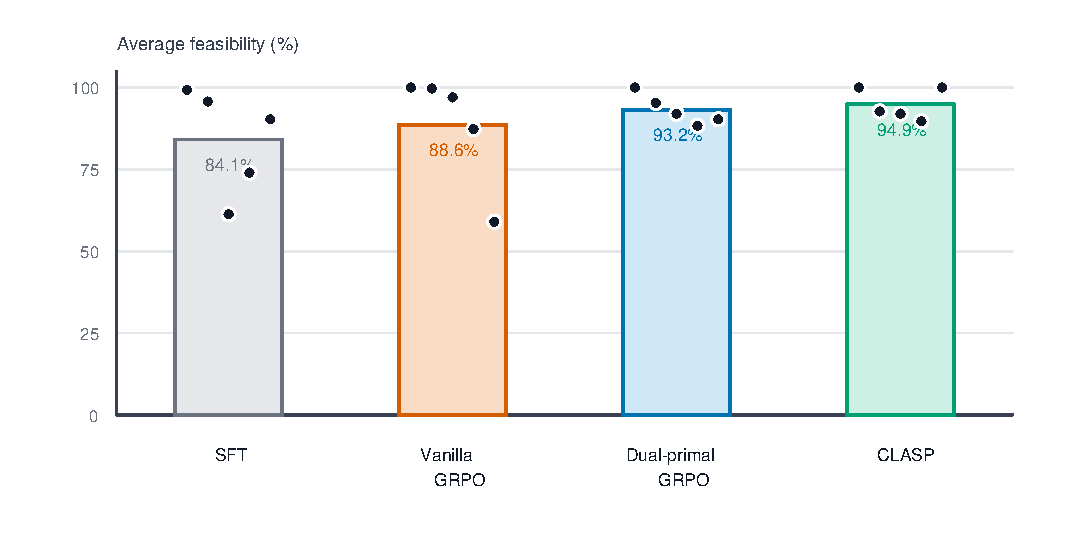
\includegraphics[width=0.58\linewidth]{figs/fig08_ablation_average_feasibility_bar.pdf}
  \caption{Average feasibility across the main training variants. Higher is better. The plotted comparison includes SFT, vanilla GRPO, Dual-primal GRPO, and CLASP; it should be read together with the main hard-group diagnostic in Figure~\ref{fig:hard_group_main}, rather than as a complete factorial ablation suite.}
  \label{fig:ablation_feasibility_bar}
\end{figure}

\begin{table}[!b]
\caption{Dataset and context diagnostics for the supported five-task setup. The table highlights sequence-length pressure and split overlap for the tasks used in the experiments. The token statistics aggregate only TSP, OP, CVRP, MIS, and JSSP, and the overlap count is based on a direct audit of the provided data splits.}
\label{tab:diagnostics}
\centering
\small
\begin{tabular}{lc}
\toprule
Diagnostic & Value \\
\midrule
Supported five-task combined sequences \(> 4096\) tokens & \(21.10\%\) \\
Supported five-task combined sequences \(> 8192\) tokens & \(0.88\%\) \\
Supported five-task combined sequences \(> 12288\) tokens & \(0.04\%\) \\
TSP SFT-eval / GRPO-eval exact overlap & \(300\) \\
OP/CVRP/MIS/JSSP SFT-eval / GRPO-eval overlap & \(0\) \\
\bottomrule
\end{tabular}
\end{table}

The primary training configuration uses a Qwen2.5-7B-Instruct base model with multi-node H100 GPU training, bfloat16 arithmetic, and LoRA adaptation. We keep the SFT stage fixed across methods and vary only the RL stage. In the reported five-task setup, the SFT stage uses 50{,}000 supervised examples per task, compared with 500{,}000 in the reproduced Jiang et al. reference setting. Table~\ref{tab:rl_hparams} reports the SFT initialization and the RL-stage hyperparameters that control the CLASP grouped advantage, controller dynamics, and adaptive length mechanism.

\begin{table*}[t]
\caption{Core training hyperparameters for the reported five-task CLASP configuration. The same rollout group size, batch settings, optimizer-facing overrides, and decoding cap are used for internal RL baselines; the length-normalized sequence surrogate is fixed across constrained variants unless a variant explicitly changes that component.}
\label{tab:rl_hparams}
\centering
\small
\begin{tabularx}{\textwidth}{lX}
\toprule
Category & Value \\
\midrule
SFT initialization & Qwen2.5-7B-Instruct; bfloat16 arithmetic; no-reason Alpaca prompt style; seed \(42\); 50{,}000 supervised examples per task with evaluation ratio \(0.05\); LoRA rank \(64\), LoRA \(\alpha=64\), LoRA dropout \(0\); learning rate \(2\times 10^{-4}\); \(5\) epochs; context window / maximum sequence length \(8192\); per-device train/eval batch \(2/1\), effective optimization batch \(64\) on \(32\) H100 GPUs. \\
RL model and adaptation & Initialized from the fixed SFT checkpoint; bfloat16 arithmetic; no-reason Alpaca prompt style; seed \(42\); full finetuning disabled; LoRA rank \(64\), LoRA \(\alpha=64\), LoRA dropout \(0\); learning rate \(10^{-6}\); \(20\) epochs. \\
Rollouts and surrogate & Rollout group size \(K=8\); per-device train/eval batch \(4/4\); gradient accumulation \(4\), effective optimization batch \(256\) on \(16\) H100 GPUs; generation batch \(512\); maximum prompt length \(7168\); maximum completion length \(L_{\max}=1024\); context window \(8192\); constrained variants use the length-normalized sequence surrogate from Eq.~\eqref{eq:seqratio} and PPO-style clipping as in Eq.~\eqref{eq:clipsurrogate}, with no additional reward scaling. \\
Trainer defaults & Other trainer hyperparameters not overridden by the launchers, including optimizer type, scheduler, Adam coefficients, weight decay, gradient clipping, and PPO clipping constants, follow the TRL/Transformers defaults for the recorded TRL \(0.24.0\), Transformers \(4.57.3\), and Accelerate \(1.12.0\) environment. \\
CLASP grouped advantage and reward gate & Feasibility transition sharpness \(\beta=4.0\); within-group standard-deviation stabilizer \(\varepsilon=10^{-4}\); primal weight \(w_o=1.0\); structure weight \(w_s=0.3\); infeasible partial-credit gate from Eq.~\eqref{eq:softgate} enabled. \\
Controller & Base controller step size \(\eta_0=0.0075\); controller refresh period \(n_\lambda=4\) primal optimizer steps; \(\lambda_0=0\); \(\lambda_{\max}=1.0\); feasibility-conditioned step-size stabilizer \(\varepsilon=10^{-3}\). \\
Dense-cost thresholds & Global controller cost limit \(0.03\); violation tolerance \(0.01\); task-component tolerances are listed in Appendix~\ref{app:costs}. \\
Adaptive length & Enabled; rolling-window size \(1000\); quantile \(q=0.99\); floor \(L_{\min}=128\); refresh period \(R=50\) optimizer steps. \\
\bottomrule
\end{tabularx}
\end{table*}

Some implementation flags and historical ablation logs retain early names such as \texttt{clasp\_pareto\_tau} and \texttt{clasp\_pareto\_anchor} for checkpoint and script compatibility. In the notation of this paper, \texttt{clasp\_pareto\_tau} is the transition-sharpness parameter \(\beta\), and disabling the historical \texttt{clasp\_pareto\_anchor} flag disables the adaptive grouped advantage in Eq.~\eqref{eq:claspadv}; no Pareto anchor enters the mathematical grouped advantage.

Evaluation uses the same prompt template, parsers, and thresholded feasibility checks as training-time reward computation, but every candidate is rescored from its parsed discrete structure. For best-of-\(N\) decoding, we select the feasible candidate with the lowest recomputed reference gap for each instance; ties are broken by lower violation and then by the earliest sampled candidate. Instances with no feasible candidate contribute to feasibility and Success@\(k\) rates but are excluded from mean and median best-feasible gap summaries. We avoid assigning infeasible instances an arbitrary penalized optimality gap; when feasibility differs sharply, Success@\(k\) and feasibility are the fair all-instance comparisons, while best-feasible gap is a conditional quality diagnostic.

\clearpage
\section{Additional Reference Results and Diagnostics}
\label{app:additional_results}

Figure~\ref{fig:pipeline} provides a compact visual summary of the CLASP-GRPO training loop. Figures~\ref{fig:ablation_feasibility_bar} and \ref{fig:inference_hard_group_recovery} move supporting mechanism summaries out of the main text: the former reports the training-variant feasibility comparison, and the latter shows recovery on prompts where classic GRPO produced no feasible candidate. Figure~\ref{fig:jssp_bon_ablation_appendix} adds a JSSP best-of-\(N\) ablation that varies the candidate budget to show how feasibility and reference-gap change with larger decoding pools. The additional mechanism diagnostics in Figures~\ref{fig:all_infeasible_frequency} and \ref{fig:mechanism_dashboard} show how often hard all-infeasible groups arise and how the grouped advantage and controller behave, while Figure~\ref{fig:curves} compares CLASP against Dual-primal GRPO over training.

\begin{figure}[t]
  \centering
  \fbox{%
  \begin{minipage}{0.93\linewidth}
  \small
  \centering
  Prompted CO instance \(x\) \\
  \(\downarrow\) shared decoder-only policy \(\pi_\theta\) \\
  \(K\) sampled completions \(\{y_i\}_{i=1}^K\) \\
  \(\downarrow\) parse and task-specific feasibility checks \\
  \begin{tabular}{c@{\hspace{1.5cm}}c}
  structure/objective rewards & dense costs and masks \\
  \(s_i, o_i\) & \(\mathbf{c}_i^{(\tau)}, \mathbf{m}_i^{(\tau)}\)
  \end{tabular} \\
  \(\downarrow\) \\
  feasibility rate and group statistics \\
  \(\downarrow\) \\
  CLASP grouped advantage \(A_i^{\mathrm{CLASP}}\) from Eq.~\eqref{eq:claspadv} \\
  \(\downarrow\) \\
  clipped policy update \hspace{1cm} feasibility-conditional controller update
  \end{minipage}}
  \caption{Overview of CLASP-GRPO, highlighting the adaptive centered within-group advantage, taskwise signed-gap controller, and adaptive decoding budget.}
  \label{fig:pipeline}
\end{figure}

\begin{figure}[t]
  \centering
  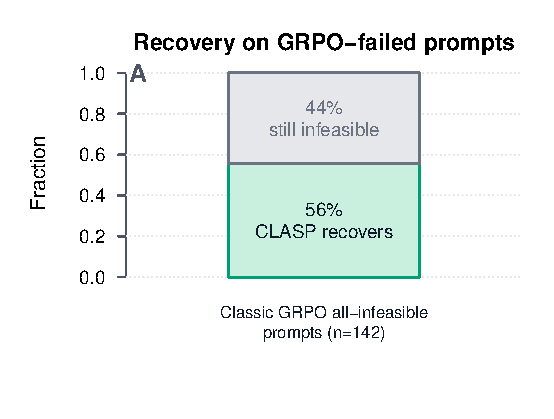
\includegraphics[width=0.5\linewidth]{figs/fig_inference_hard_group_recovery_appendix.pdf}
  \caption{Recovery on prompts where classic GRPO produced no feasible candidate. The denominator is the \(142\) hard-split prompts for which all \(K=8\) classic GRPO candidates were infeasible; CLASP recovers at least one feasible candidate on \(55.6\%\) of them.}
  \label{fig:inference_hard_group_recovery}
\end{figure}

\begin{figure}[t]
  \centering
  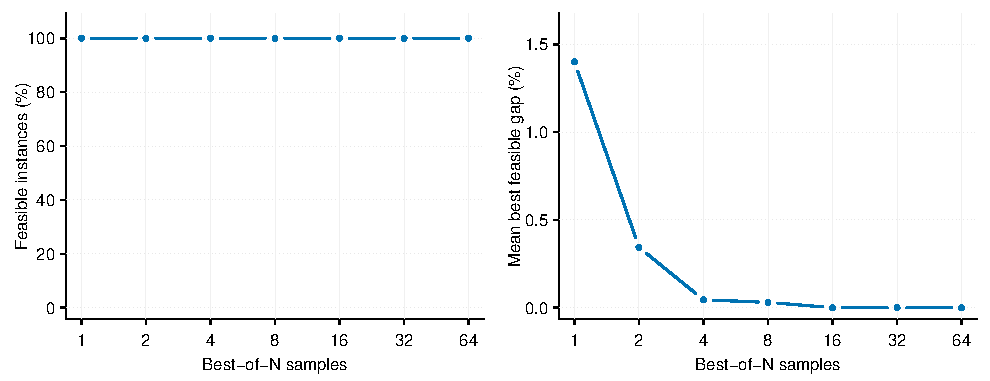
\includegraphics[width=0.72\linewidth]{figs/fig_jssp_bon1_to_64_feasibility_gap.pdf}
  \caption{JSSP best-of-\(N\) ablation with varying candidate budget \(N\). The plot reports how feasibility and conditional reference-value gap change as the best-of-\(N\) decoding budget increases from 1 to 64, providing appendix-level context for the BoN sensitivity of the JSSP results.}
  \label{fig:jssp_bon_ablation_appendix}
\end{figure}

\begin{figure}[t]
  \centering
  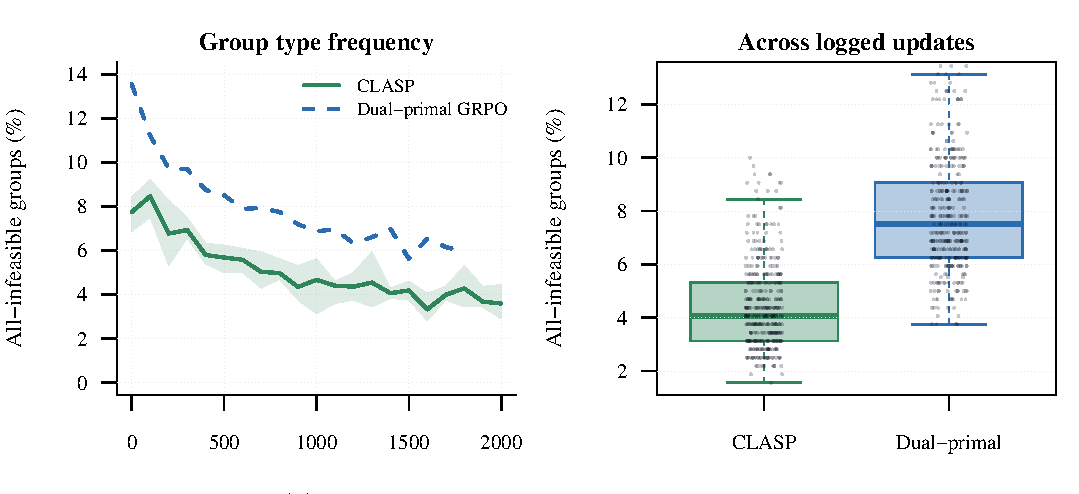
\includegraphics[width=0.9\linewidth]{figs/app_mech01_all_infeasible_frequency.pdf}
  \caption{Frequency of hard prompt groups during training. Left: the fraction of all-infeasible groups over RL steps for CLASP and the Dual-primal GRPO baseline. Right: summary distribution of the all-infeasible-group rates across logged updates. The figure supports the motivating claim that hard prompts frequently induce all-infeasible groups and shows how the learned policies differ in that regime.}
  \label{fig:all_infeasible_frequency}
\end{figure}

\begin{figure}[t]
  \centering
  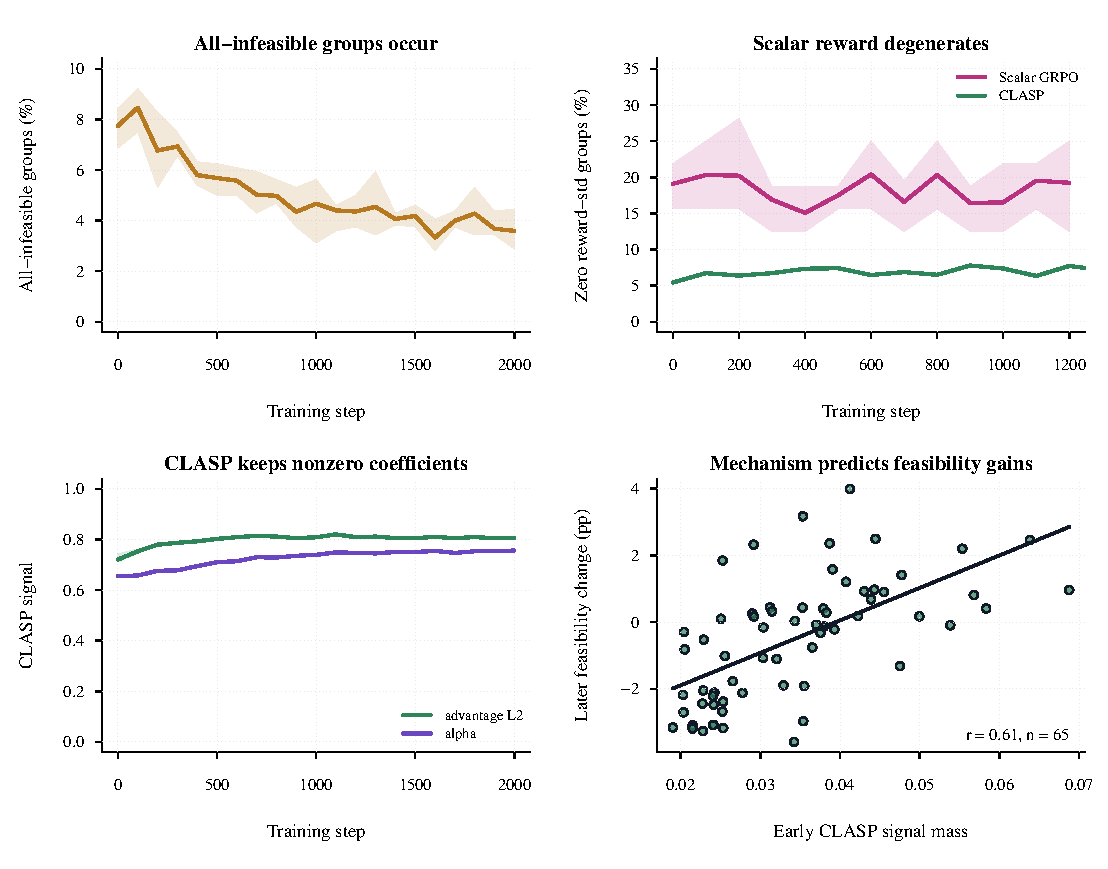
\includegraphics[width=0.95\linewidth]{figs/app_mech00_mechanism_dashboard.pdf}
  \caption{Mechanism diagnostics for CLASP. The panels summarize group-level failure modes and controller behavior, including all-infeasible-group prevalence, scalar-reward degeneracy, grouped-advantage evolution, and the relation between early CLASP gap reduction and later feasible-quality gains. Together they provide appendix-level evidence for the mechanism discussion in Section~\ref{sec:method}.}
  \label{fig:mechanism_dashboard}
\end{figure}

\begin{figure}[p]
  \centering
  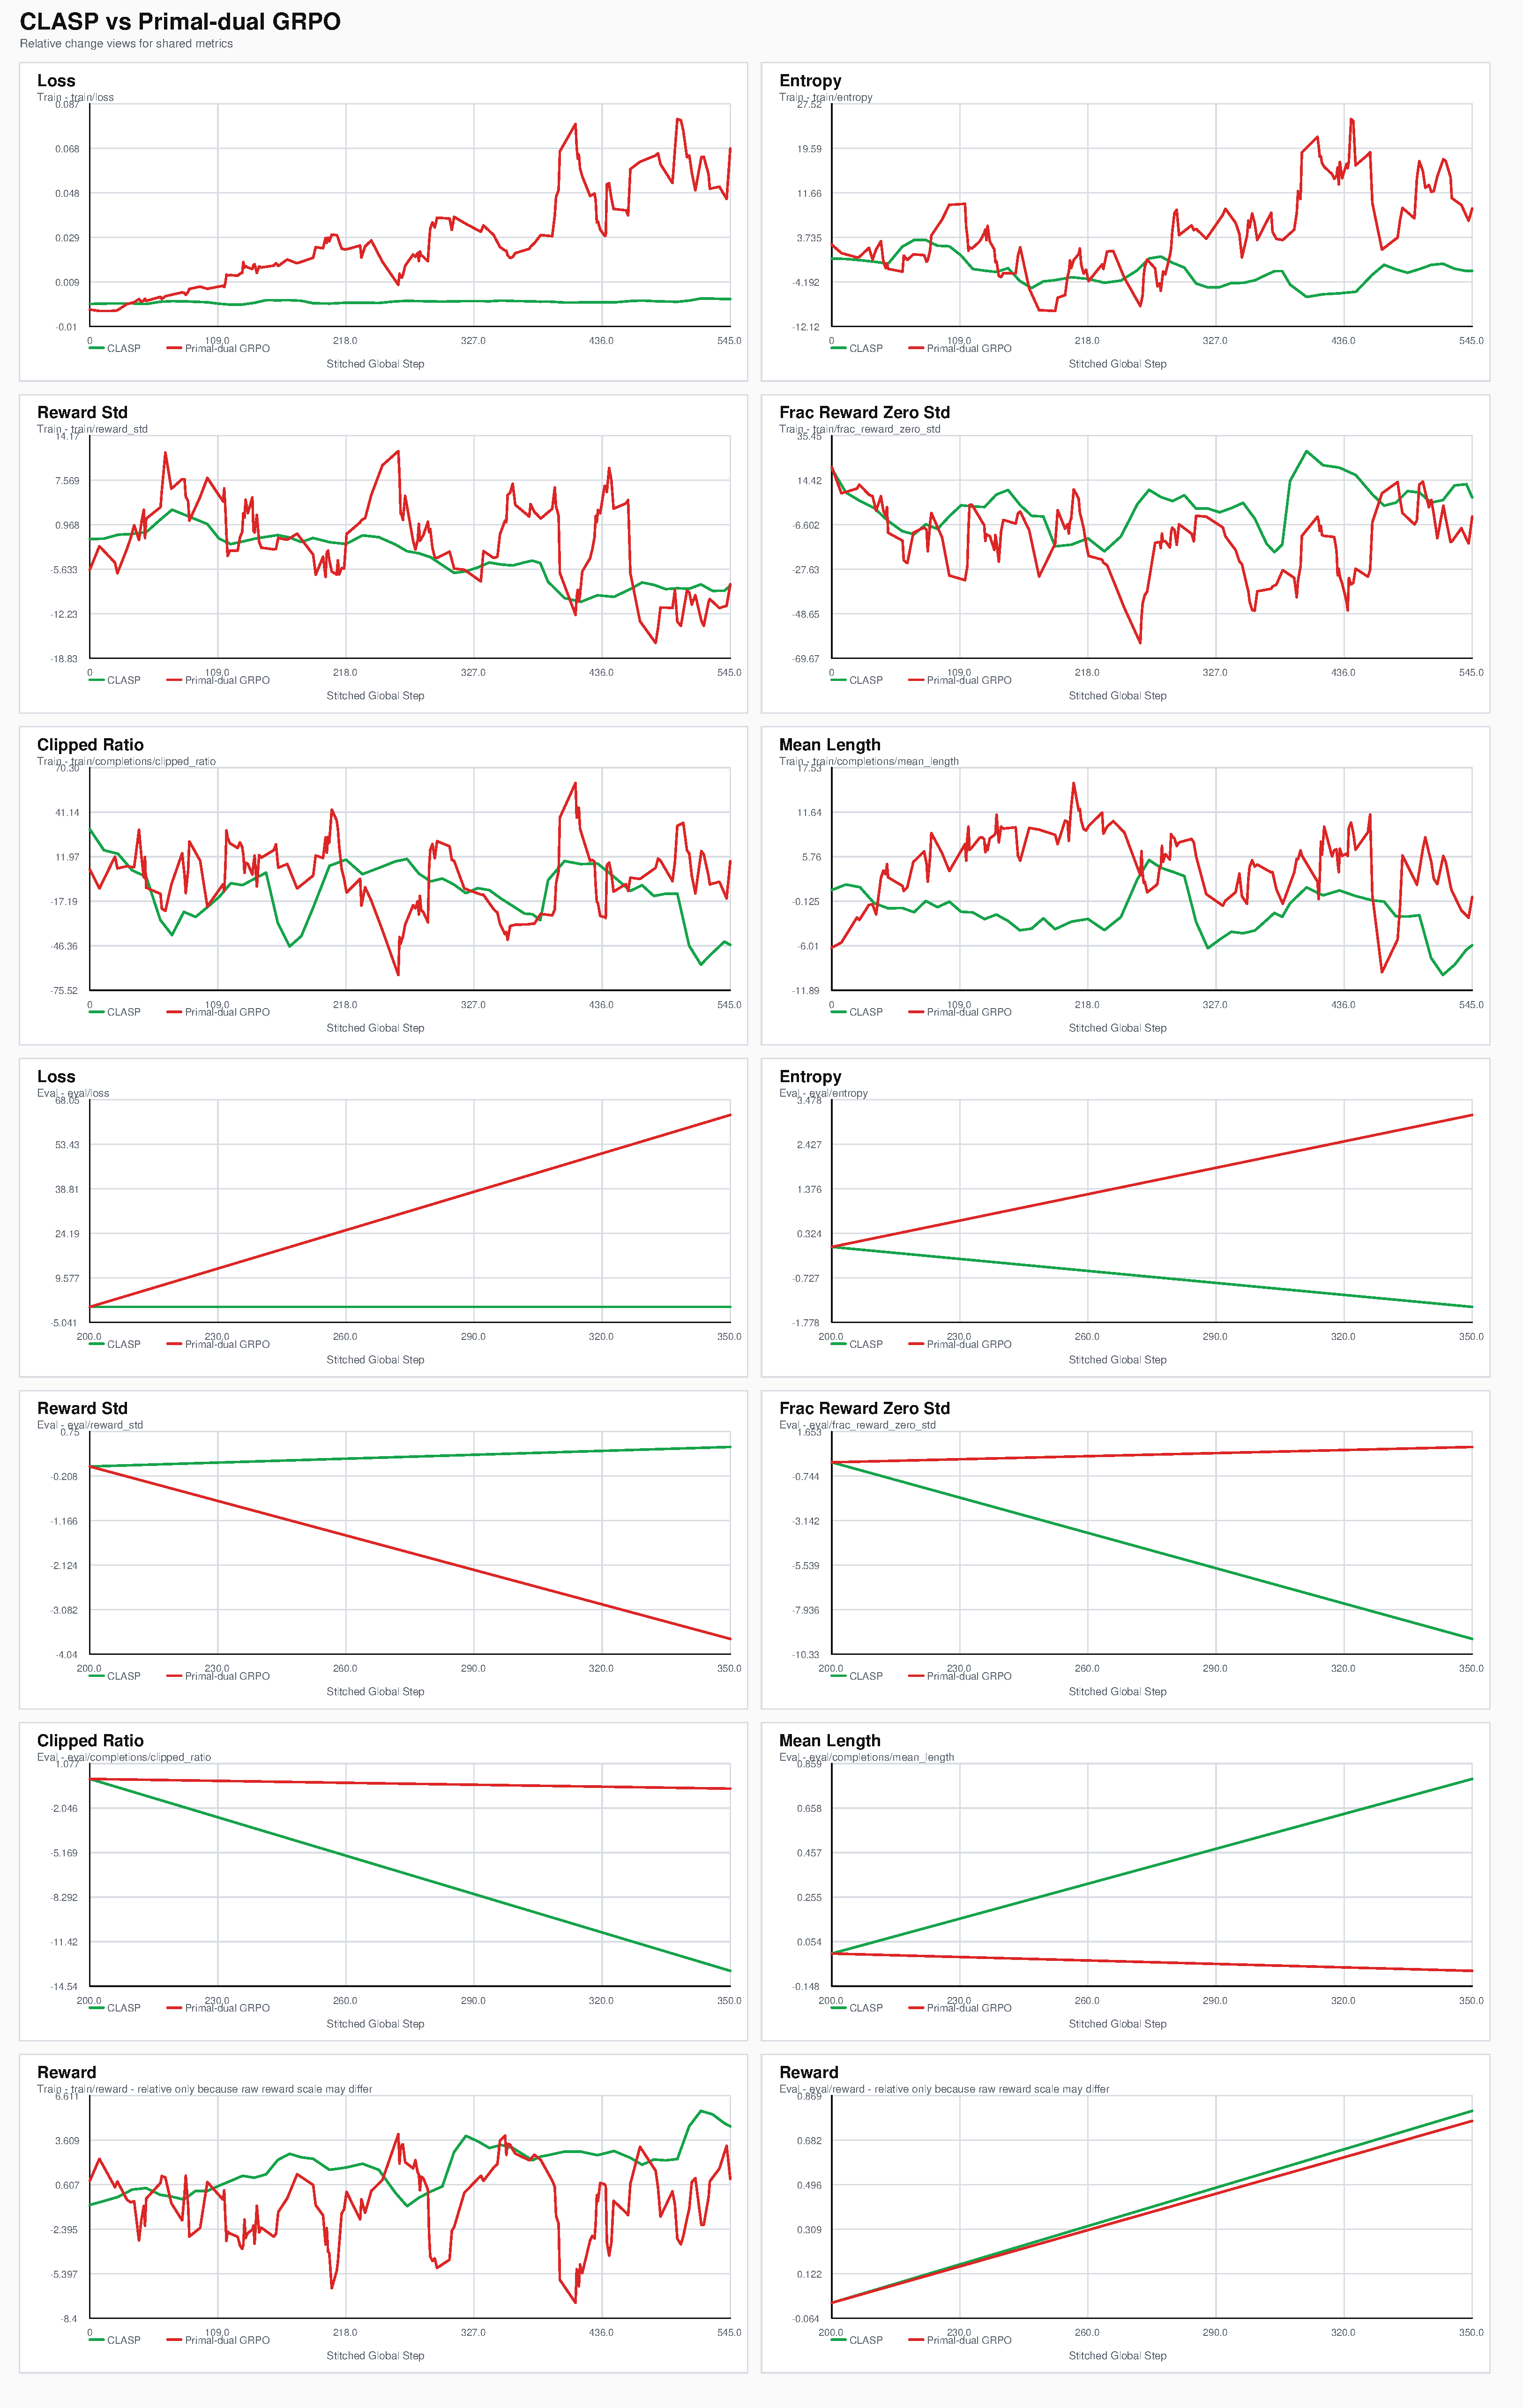
\includegraphics[width=0.88\linewidth]{figs/app_train07_clasp_vs_dual_primal_relative.pdf}
  \caption{Training-dynamics comparison between CLASP and Dual-primal GRPO. The panels track relative trends in feasibility, feasible quality, controller values, and related diagnostics over optimization. This figure is included in the appendix because it is useful for attribution and reviewer inspection, but too dense for the main paper.}
  \label{fig:curves}
\end{figure}

\section{Task-Specific Dense Cost Components}
\label{app:costs}
The dense cost vectors used in this work are:
\sloppy
\begin{itemize}
\item \textbf{TSP}: \texttt{parse\_failure}, \texttt{depot\_boundary}, \texttt{invalid\_node}, \texttt{duplicate\_customer}, \texttt{missing\_customer}, \texttt{interior\_depot}.
\item \textbf{CVRP}: \texttt{parse\_failure}, \texttt{route\_count\_mismatch}, \texttt{depot\_boundary}, \texttt{invalid\_node}, \texttt{duplicate\_customer}, \texttt{missing\_customer}, \texttt{interior\_depot}, \texttt{capacity\_overflow}.
\item \textbf{OP}: \texttt{parse\_failure}, \texttt{start\_at\_depot}, \texttt{invalid\_node}, \texttt{duplicate\_visit}, \texttt{length\_overflow}.
\item \textbf{MIS}: \texttt{parse\_failure}, \texttt{invalid\_node}, \texttt{duplicate\_node}, \texttt{edge\_conflict}.
\item \textbf{JSSP}: \texttt{parse\_failure}, \texttt{machine\_row\_mismatch}, \texttt{row\_length\_mismatch}, \texttt{duplicate\_job}, \texttt{missing\_job}, \texttt{schedule\_invalid}.
\end{itemize}
\fussy
Every cost is clipped into \([0,1]\), every mask is binary, and every sample must expose at least one active component.
\begin{sloppypar}
\begin{itemize}
\item Tolerances use \(\epsilon_j=0\) for \texttt{parse\_failure}, \texttt{depot\_boundary}, \texttt{start\_at\_depot}, \texttt{invalid\_node}, \texttt{duplicate\_customer}, \texttt{missing\_customer}, \texttt{duplicate\_visit}, \texttt{duplicate\_node}, \texttt{edge\_conflict}, \texttt{machine\_row\_mismatch}, \texttt{row\_length\_mismatch}, \texttt{duplicate\_job}, \texttt{missing\_job}, \texttt{schedule\_invalid}, and \texttt{interior\_depot}; \(\epsilon_j=0.02\) for \texttt{route\_count\_mismatch} and \texttt{capacity\_overflow}; and \(\epsilon_j=0.015\) for \texttt{length\_overflow}.
\item The binary feasibility flag is set to one only when the maximum positive component gap is at most \(10^{-8}\).
\item The \texttt{co\_default} weights are \(5.0\) for \texttt{parse\_failure}, \texttt{missing\_customer}, and \texttt{edge\_conflict}; \(4.0\) for \texttt{invalid\_node}; \(3.5\) for \texttt{depot\_boundary}, \texttt{start\_at\_depot}, \texttt{machine\_row\_mismatch}, \texttt{row\_length\_mismatch}, and \texttt{duplicate\_job}; \(2.5\) for \texttt{interior\_depot}; \(1.5\) for \texttt{route\_count\_mismatch} and \texttt{duplicate\_node}; \(3.0\) for \texttt{capacity\_overflow} and \texttt{length\_overflow}; \(2.0\) for \texttt{duplicate\_visit}; and \(4.5\) for \texttt{missing\_job}.
\item Task-specific overrides use \(6.0\) for CVRP \texttt{missing\_customer}, MIS \texttt{edge\_conflict}, and JSSP \texttt{schedule\_invalid}; \(5.0\) for CVRP \texttt{duplicate\_customer} and JSSP \texttt{missing\_job}; \(4.0\) for CVRP \texttt{capacity\_overflow}, CVRP \texttt{depot\_boundary}, OP \texttt{length\_overflow}, and OP \texttt{start\_at\_depot}; and \(1.0\) for MIS \texttt{duplicate\_node}.
\end{itemize}
\end{sloppypar}
Under the mask-completeness assumption, the controller therefore always observes some task-defined violation information, even for malformed outputs.

For monitoring only, we also log the scalar diagnostic summary
\begin{align}
\mathrm{constraint}_i = 1 - \frac{1}{|\{j:m_{ij}^{(\tau)}=1\}|}\sum_{j:m_{ij}^{(\tau)}=1} c_{ij}^{(\tau)},
\end{align}
which is well-defined because every sample exposes at least one active component. This diagnostic is not used in either the CLASP grouped advantage or the controller update.

\section{Formal Arguments and Proofs}
\label{app:formal}

\begin{proposition}[Population constraints align with thresholded feasibility]
\label{prop:population-feasibility}
Fix a task \(\tau\) and assume the mask family is complete for the task semantics. For each component \(j\), define
\begin{align}
V_{\tau,j}(\theta)
=
\mathbb{E}_{x\sim\mathcal D_\tau,\,y\sim\pi_\theta(\cdot\mid x)}
\Bigl[m_j^{(\tau)}(x,y)\max\!\left\{0,c_j^{(\tau)}(x,y)-\epsilon_j^{(\tau)}\right\}\Bigr].
\end{align}
Then \(V_{\tau,j}(\theta)\ge 0\) for every \(j\), and the conjunction \(V_{\tau,j}(\theta)=0\) for all active task components is equivalent to almost-sure thresholded feasibility of the sampled completions with respect to the dense costs and tolerances, i.e.,
\begin{align}
\sum_{j=1}^{m_\tau} m_j^{(\tau)}(x,y)\max\!\left\{0,c_j^{(\tau)}(x,y)-\epsilon_j^{(\tau)}\right\}=0
\quad \text{for } \mathcal D_\tau\otimes\pi_\theta\text{-almost every }(x,y).
\end{align}
Under mask completeness, this almost-sure condition coincides with thresholded feasibility for all semantically applicable violation types.
\end{proposition}

\begin{proposition}[Centered CLASP grouped advantages are well-defined]
\label{prop:clasp-well-defined}
For every finite prompt group \(G=\{(r_i,g_i(\boldsymbol{\lambda}),v_i)\}_{i=1}^K\) with \(K \ge 1\), finite \(r_i\) and \(g_i(\boldsymbol{\lambda})\), well-defined feasibility indicators \(\mathbf{1}[v_i=0]\), \(\beta\in(0,\infty)\), and \(\varepsilon>0\), the CLASP grouped advantages in Eq.~\eqref{eq:claspadv} are finite and satisfy \(\sum_{i=1}^K A_i^{\mathrm{CLASP}}=0\).
\end{proposition}

\begin{remark}[Reference-sample cancellation]
\label{rem:reference-cancellation}
For any group-level reference index \(a\in[K]\), including one selected from a Pareto frontier or any other deterministic rule, define the raw reference advantage
\begin{align}
\widetilde A_i(a)
=
\alpha_G\frac{r_i-r_a}{\sigma_r^G+\varepsilon}
+
(1-\alpha_G)\frac{g_a(\boldsymbol{\lambda})-g_i(\boldsymbol{\lambda})}{\sigma_g^G+\varepsilon}.
\end{align}
Its within-group centered form is independent of \(a\):
\begin{align}
\widetilde A_i(a)
-
\frac{1}{K}\sum_{k=1}^K\widetilde A_k(a)
=
\alpha_G\frac{r_i-\bar r_G}{\sigma_r^G+\varepsilon}
+
(1-\alpha_G)\frac{\bar g_G-g_i(\boldsymbol{\lambda})}{\sigma_g^G+\varepsilon}
=
A_i^{\mathrm{CLASP}}.
\end{align}
Thus no reference sample enters the mathematical grouped advantage in Eq.~\eqref{eq:claspadv}; historical implementation names involving ``anchor'' refer to enabling or disabling the whole centered grouped advantage.
\end{remark}

\begin{proposition}[Projected CLASP controller fixed-point conditions]
\label{prop:controller-fixed-point}
Fix a task \(\tau\) and freeze \(\theta\). Consider the deterministic controller obtained by replacing minibatch statistics with their expectations, and assume the signed moment \(G_{\tau,j}(\theta)\) is finite:
\begin{align}
F_\tau(\theta) &= \mathbb{E}_{x \sim \mathcal D_\tau,\, y \sim \pi_\theta(\cdot\mid x)}\bigl[\mathbf{1}[v(x,y) = 0]\bigr], \\
\lambda_{t+1,j}
&=
\Pi_{[0,\lambda_{\max}]}
\left(
\lambda_{t,j}
+
\eta_0 \sqrt{\frac{1-F_\tau(\theta)+\varepsilon}{F_\tau(\theta)+\varepsilon}}\, G_{\tau,j}(\theta)
\right),
\end{align}
where \(\eta_0>0\), \(\varepsilon>0\), \(\lambda_{\max}>0\), and \(\Pi_{[0,\lambda_{\max}]}\) denotes Euclidean projection onto \([0,\lambda_{\max}]\). Any fixed point \(\lambda_j^\star\) satisfies the sign conditions
\begin{align}
0 < \lambda_j^{\star} < \lambda_{\max}
&\implies
G_{\tau,j}(\theta)=0, \\
\lambda_j^{\star} = 0
&\implies
G_{\tau,j}(\theta)\le 0, \\
\lambda_j^{\star} = \lambda_{\max}
&\implies
G_{\tau,j}(\theta)\ge 0.
\end{align}
\end{proposition}

\begin{theorem}[Non-degeneracy of the CLASP grouped advantage in the constant-primal all-infeasible regime]
\label{thm:clasp-nondegenerate}
Let \(G=\{(r_i,g_i(\boldsymbol{\lambda}),v_i)\}_{i=1}^K\) be a finite prompt group with \(K\ge 2\) and finite real-valued primal scores and controller-weighted gaps. Assume that:
\begin{enumerate}
\item every completion in the group is infeasible, so \(v_i>0\) for all \(i\in[K]\);
\item the primal scores are constant across the group, so \(r_i=r_\circ\) for all \(i\in[K]\);
\item the controller-weighted feasibility gaps are not constant across the group, so there exist \(i,j\in[K]\) with \(g_i(\boldsymbol{\lambda})\neq g_j(\boldsymbol{\lambda})\);
\item The dense-rank and recovery estimators use finite positive stabilizers and bounded rank scores, so their centered group credits are finite.
\end{enumerate}
Then the centered grouped advantages \((A_i^{\mathrm{CLASP}})_{i=1}^K\) defined in Eq.~\eqref{eq:claspadv} are well-defined, sum to zero, and are not identically zero. By contrast, any mean-centered scalar-reward advantage based only on \((r_i)_{i=1}^K\) and proportional to \(r_i-\bar r_G\), including the stabilized standardized quantity \((r_i-\bar r_G)/(\sigma_r^G+\varepsilon)\), is identically zero on the same group.
\end{theorem}

\begin{proof}[Proof of Theorem~\ref{thm:clasp-nondegenerate}]
By Proposition~\ref{prop:clasp-well-defined}, the CLASP grouped advantages are finite and sum to zero. Because every completion is infeasible, \(f_G=0\), so \(\alpha_G=\sigma(-\beta/2)\in(0,1)\) for every finite \(\beta>0\). Because the primal scores are constant across the group, \(\bar r_G=r_\circ\), \(\sigma_r^G=0\), and the primal contribution to Eq.~\eqref{eq:claspadv} is identically zero. Because the controller-weighted gaps are not constant, \(\sigma_g^G>0\).

Therefore the CLASP grouped advantages reduce to
\begin{align}
A_i^{\mathrm{CLASP}}
=
(1-\alpha_G)
\frac{\bar g_G-g_i(\boldsymbol{\lambda})}{\sigma_g^G+\varepsilon}.
\end{align}
Since \((g_i(\boldsymbol{\lambda}))_{i=1}^K\) is not constant, at least one \(g_i(\boldsymbol{\lambda})\) differs from \(\bar g_G\). For that index, \(A_i^{\mathrm{CLASP}}\neq 0\) because \(1-\alpha_G>0\) and \(\sigma_g^G+\varepsilon>0\). By contrast, the primal scores are constant, so \(r_i-\bar r_G=0\) for every \(i\). Hence every mean-centered scalar-reward advantage proportional to \(r_i-\bar r_G\), including \((r_i-\bar r_G)/(\sigma_r^G+\varepsilon)\), is identically zero. Therefore \(A^{\mathrm{CLASP}}\) is well-defined, zero-sum, and non-trivial, whereas the centered scalar baseline is degenerate on the same group.
\end{proof}

\begin{proof}[Proof of Proposition~\ref{prop:population-feasibility}]
Each integrand in \(V_{\tau,j}(\theta)\) is nonnegative, so \(V_{\tau,j}(\theta)\ge 0\). If \(V_{\tau,j}(\theta)=0\), then the nonnegative random variable
\begin{align}
Z_{\tau,j}(x,y)=m_j^{(\tau)}(x,y)\max\!\left\{0,c_j^{(\tau)}(x,y)-\epsilon_j^{(\tau)}\right\}
\end{align}
has zero expectation and therefore vanishes for \(\mathcal D_\tau\otimes\pi_\theta\)-almost every \((x,y)\). If this holds for every active component \(j\), then the finite sum of these nonnegative terms also vanishes almost surely, which is exactly the displayed thresholded-feasibility condition. Conversely, if the summed thresholded-feasibility condition holds almost surely, then each nonnegative summand must vanish almost surely, implying \(V_{\tau,j}(\theta)=0\) for every \(j\). Under mask completeness, every semantically applicable violation type is represented by an active mask entry and corresponding dense cost, so this almost-sure vanishing condition coincides with thresholded feasibility for all semantically applicable violation types.
\end{proof}

\begin{proof}[Proof of Proposition~\ref{prop:clasp-well-defined}]
The logistic sigmoid maps the finite argument \(\beta(f_G-1/2)\) to a finite \(\alpha_G\in(0,1)\). The denominators \(\sigma_r^G+\varepsilon\) and \(\sigma_g^G+\varepsilon\) are strictly positive because empirical standard deviations are nonnegative and \(\varepsilon>0\). Thus each grouped advantage in Eq.~\eqref{eq:claspadv} is finite whenever the group scores are finite. Moreover,
\begin{align}
\sum_{i=1}^K (r_i-\bar r_G)=0,
\qquad
\sum_{i=1}^K (\bar g_G-g_i(\boldsymbol{\lambda}))=0.
\end{align}
Multiplying these two zero sums by the group-constant factors in Eq.~\eqref{eq:claspadv} gives \(\sum_{i=1}^K A_i^{\mathrm{CLASP}}=0\).
\end{proof}

\begin{proof}[Proof of Proposition~\ref{prop:controller-fixed-point}]
Fix a component \(j\). The scalar factor
\begin{align}
\kappa_\tau(\theta)=\eta_0 \sqrt{\frac{1-F_\tau(\theta)+\varepsilon}{F_\tau(\theta)+\varepsilon}}
\end{align}
is finite and strictly positive: \(F_\tau(\theta)\in[0,1]\) because it is an expectation of an indicator, while \(\eta_0>0\) and \(\varepsilon>0\). At a fixed point,
\begin{align}
\lambda_j^\star
=
\Pi_{[0,\lambda_{\max}]}
\left(
\lambda_j^\star + \kappa_\tau(\theta) G_{\tau,j}(\theta)
\right).
\label{eq:fixedpoint-clasp}
\end{align}
If \(0<\lambda_j^\star<\lambda_{\max}\), the projection is inactive at \(\lambda_j^\star\), so Eq.~\eqref{eq:fixedpoint-clasp} implies \(\kappa_\tau(\theta) G_{\tau,j}(\theta)=0\). Since \(\kappa_\tau(\theta)>0\), we obtain \(G_{\tau,j}(\theta)=0\).

If \(\lambda_j^\star=0\), Eq.~\eqref{eq:fixedpoint-clasp} can hold only if the quantity inside the projection is non-positive. That is, \(\kappa_\tau(\theta) G_{\tau,j}(\theta)\le 0\). Positivity of \(\kappa_\tau(\theta)\) then gives \(G_{\tau,j}(\theta)\le 0\).

If \(\lambda_j^\star=\lambda_{\max}\), the quantity inside the projection must be at least \(\lambda_{\max}\), which implies \(\kappa_\tau(\theta) G_{\tau,j}(\theta)\ge 0\). Again \(\kappa_\tau(\theta)>0\), so \(G_{\tau,j}(\theta)\ge 0\). This proves the stated complementary-sign conditions.
\end{proof}

\FloatBarrier
\section{Appendix Discussion and Supplemental Tables}
\label{app:appendix_discussion}
Tables~\ref{tab:ta_subset}, \ref{tab:tsplib_gap_comparison_clasp}, \ref{tab:performance_comparison}, and \ref{tab:solving_time} provide a compact appendix-level view of how the proposed method compares under four complementary lenses. Table~\ref{tab:ta_subset} shows that the matched Taillard-format JSSP comparison remains competitive but still sensitive to evaluation protocol and candidate budget, so we interpret it as a targeted external reference rather than a standalone headline result. Figure~\ref{fig:jssp_bon_ablation_appendix} complements that table with a JSSP BoN ablation study over varying \(N\), highlighting how larger decoding budgets affect feasibility and gap. Table~\ref{tab:tsplib_gap_comparison_clasp} adds a TSPLIB TSP comparison against prior LLM-based methods and shows that increasing CLASP's best-of-\(N\) budget substantially narrows the gap.

Tables~\ref{tab:performance_comparison} and \ref{tab:solving_time} summarize the broader positioning of CLASP across problems and runtime. Together they show that CLASP remains a fast learned policy and matches or improves the Jiang et al. best-of-\(N\) reference gaps across the five shared tasks under the current protocol. They also show that CLASP preserves the fast policy-decoding profile of the underlying SFT/RL model, even when it is modestly slower than the lightest open-weight general-purpose models on some tasks.

\begin{table*}[!ht]
\caption{Reference comparison on Taillard-format JSSP instances from \citet{jiang2025endtoendco}. Lower objective value and lower relative gap indicate better performance. Rows labeled ``Jiang et al.'' correspond to entries labeled ``Ours'' in the source paper, and asterisks follow the source notation. Comparisons should be interpreted only under matched \(N\) and evaluation protocol.``Adj.-swap polish'' denotes a deterministic post-processing step that starts from the best feasible BoN schedule and greedily applies adjacent swaps in machine-order lists whenever the swap reduces the JSSP makespan.}
\label{tab:ta_subset}
\centering
\scriptsize
\resizebox{0.9\textwidth}{!}{%
\begin{tabular}{lcccccc}
\toprule
Method & \multicolumn{2}{c}{TA 15x15} & \multicolumn{2}{c}{TA 20x15} & \multicolumn{2}{c}{TA 20x20} \\
\cmidrule(lr){2-3}\cmidrule(lr){4-5}\cmidrule(lr){6-7}
 & obj.$\downarrow$ & opt.$\downarrow$ & obj.$\downarrow$ & opt.$\downarrow$ & obj.$\downarrow$ & opt.$\downarrow$ \\
\midrule
Best-known solution & 1228.9 & -- & 1364.9 & -- & 1617.3 & -- \\
SPT & 1546.1 & 25.81\% & 1813.5 & 32.87\% & 2067.2 & 27.81\% \\
FIFO & 1657.4 & 34.87\% & 2008.4 & 47.15\% & 2297.1 & 42.03\% \\
ATC & 1586.8 & 29.12\% & 1794.3 & 31.46\% & 2114.1 & 30.72\% \\
GA* 100x100 & 1583.8 & 28.88\% & 1847.1 & 35.23\% & 2304.2 & 42.47\% \\
L2D greedy & 1522.3 & 23.88\% & 1813.4 & 32.86\% & 2130.2 & 31.21\% \\
L2D sample & 1543.8 & 25.62\% & 1779.7 & 30.39\% & 2134.2 & 31.96\% \\
StarJob* & -- & 19.68\% & -- & 26.91\% & -- & 33.12\% \\
Jiang et al. (N = 8) & 1403.6 & 14.22\% & 1653.7 & 21.16\% & 1994.2 & 23.30\% \\
Jiang et al. (N = 64) & 1368.2 & 11.34\% & 1600.5 & 17.26\% & 1940.9 & 20.01\% \\
CLASP (N = 8) & 1410.6 & 14.79\% & 1666.2 & 22.00\% & 2038.0 & 25.80\% \\
CLASP (N = 64) & 1402.9 & 14.16\% & 1643.4 & 20.32\% & 2009.8 & 24.06\% \\
CLASP + adj.-swap polish $(N=64)$ & \textbf{1357.7} & \textbf{10.48\%} & \textbf{1554.0} & \textbf{13.85\%} & \textbf{1907.1} & \textbf{17.92\%} \\


\bottomrule
\end{tabular}%
}
\end{table*}

\begin{table}[!ht]
\centering
\caption{Optimality gap comparison of LLM-based methods on TSPLIB instances. CLASP uses normalized-coordinate TSPLIB prompts; reported CLASP gaps are recomputed on the original TSPLIB coordinates with \texttt{EUC\_2D} rounded distances.}
\label{tab:tsplib_gap_comparison_clasp}
\resizebox{\linewidth}{!}{%
\begin{tabular}{lcccccc}
\toprule
Instance & AEL & ReEVO & MCTS-AHD & Jiang et al. & CLASP (BoN=8) & CLASP (BoN=64) \\
\midrule
eil51.tsp    & 10.84\% & 6.50\%  & 15.98\% & 2.02\% & 3.29\% & 1.64\% \\
berlin52.tsp & 12.91\% & 17.99\% & 7.08\%  & 4.54\% & 4.07\% & 0.08\% \\
st70.tsp     & 4.10\%  & 6.42\%  & 15.45\% & 0.00\% & 2.67\% & 0.15\% \\
eil76.tsp    & 10.26\% & 7.34\%  & 12.46\% & 2.91\% & 2.60\% & 1.12\% \\
pr76.tsp     & 9.06\%  & 12.17\% & 10.41\% & 3.87\% & 3.91\% & 2.48\% \\
\midrule
Average Gap  & 9.43\%  & 10.08\% & 12.28\% & 2.69\% & 3.31\% & 1.09\% \\
\bottomrule
\end{tabular}
}
\end{table}

\clearpage
\section{Additional Performance Comparison}
\label{app:performance-comparison}

Tables~\ref{tab:performance_comparison} and \ref{tab:solving_time} collect the cross-problem summary and the runtime comparison in one place for quick reference.

\begin{table}[!t]
\centering
\caption{Performance comparison across different optimization problems.}
\label{tab:performance_comparison}
\begin{tabular}{lccccc}
\toprule
Method & TSP & OP & CVRP & MIS & JSSP \\
\midrule
SOTA method & 0.00\% & 1.60\% & -0.19\% & 0.00\% & 2.45\% \\
Gurobi (1s)      & 5.76\% & 49.42\% & - & 2.28\% & 41.34\% \\
Gurobi (10s)     & 1.82\% & 21.96\% & 35.09\% & 0.46\% & 2.45\% \\
Jiang et al.     & 1.07\% & 1.85\% & 4.53\% & 1.04\% & 8.20\% \\
CLASP            & 1.01\% & 1.18\% & 4.18\% & 1.04\% & 8.19\% \\
\bottomrule
\end{tabular}
\end{table}



\begin{table}[!t]
\centering
\caption{Detailed average wall-clock solving time per problem instance for the evaluation setting used in the corresponding accuracy tables. Rows with best-of-\(N\) decoding, including CLASP, include decoding, parsing, rescoring, and feasible-candidate selection.}
\label{tab:solving_time}
\begin{tabular}{lccccc}
\toprule
Method & TSP & OP & CVRP & MIS & JSSP \\
\midrule
\multicolumn{6}{l}{\textbf{General-purpose Language Models}} \\
GPT-4o             & 7.5s  & 4.8s   & 6.8s   & 3.7s   & 5.8s \\
GPT-4o-mini        & 5.1s  & 2.4s   & 5.5s   & 3.2s   & 9.0s \\
Claude-3.7-Sonnet  & 6.7s  & 4.4s   & 6.7s   & 3.6s   & 9.2s \\
Claude-3.5-Haiku   & 5.0s  & 4.3s   & 3.5s   & 4.9s   & 9.0s \\
DeepSeek-V3-671B   & 33.0s & 22.8s  & 36.3s  & 20.3s  & 26.2s \\
Llama3.3-70B       & 2.6s  & 1.8s   & 2.2s   & 1.8s   & 3.1s \\
Qwen2.5-72B        & 13.5s & 13.3s  & 13.6s  & 6.9s   & 22.1s \\
\midrule
\multicolumn{6}{l}{\textbf{Reasoning Models}} \\
GPT-o3-mini        & 57.2s  & 109.8s & 60.5s  & 109.4s & 45.9s \\
GPT-o1             & 118.7s & 120.7s & 72.1s  & 293.5s & 98.2s \\
DeepSeek-R1        & 240.0s & 521.3s & 360.5s & 402.9s & 364.8s \\
\midrule
\multicolumn{6}{l}{\textbf{Prompt Strategies}} \\
OPRO               & 150.2s & 123.7s & 121.6s & 103.1s & 191.2s \\
LMEA               & 418.8s & 276.7s & 415.2s & 241.9s & 432.0s \\
PHP                & 96.1s  & 95.9s  & 104.2s & 85.3s  & 125.2s \\
SGE                & 166.9s & 234.3s & 308.8s & 163.7s & 260.5s \\
\midrule
\multicolumn{6}{l}{\textbf{Jiang et al.}} \\
SFT                & 7.0s  & 4.6s  & 6.9s  & 3.2s & 10.7s \\
SFT+RL             & 7.0s  & 4.6s  & 6.9s  & 3.2s & 10.7s \\
SFT+RL+BoN         & 11.7s & 10.8s & 11.3s & 4.0s & 20.7s \\
\midrule
CLASP              & 7.34s & 5.28s & 7.96s & 3.28s & 11.72s \\
\bottomrule
\end{tabular}
\end{table}


\FloatBarrier
\clearpage
\section*{NeurIPS Paper Checklist}

\begin{enumerate}

\item {\bf Claims}
    \item[] Question: Do the main claims made in the abstract and introduction accurately reflect the paper's contributions and scope?
    \item[] Answer: \answerYes{} % Replace by \answerYes{}, \answerNo{}, or \answerNA{}.
    \item[] Justification: Claims match the empirical and theoretical scope stated in the paper.
    \item[] Guidelines:
    \begin{itemize}
        \item The answer \answerNA{} means that the abstract and introduction do not include the claims made in the paper.
        \item The abstract and/or introduction should clearly state the claims made, including the contributions made in the paper and important assumptions and limitations. A \answerNo{} or \answerNA{} answer to this question will not be perceived well by the reviewers. 
        \item The claims made should match theoretical and experimental results, and reflect how much the results can be expected to generalize to other settings. 
        \item It is fine to include aspirational goals as motivation as long as it is clear that these goals are not attained by the paper. 
    \end{itemize}

\item {\bf Limitations}
    \item[] Question: Does the paper discuss the limitations of the work performed by the authors?
    \item[] Answer: \answerYes{} % Replace by \answerYes{}, \answerNo{}, or \answerNA{}.
    \item[] Justification: Limitations are discussed in the conclusion and scope statements.
    \item[] Guidelines:
    \begin{itemize}
        \item The answer \answerNA{} means that the paper has no limitation while the answer \answerNo{} means that the paper has limitations, but those are not discussed in the paper. 
        \item The authors are encouraged to create a separate ``Limitations'' section in their paper.
        \item The paper should point out any strong assumptions and how robust the results are to violations of these assumptions (e.g., independence assumptions, noiseless settings, model well-specification, asymptotic approximations only holding locally). The authors should reflect on how these assumptions might be violated in practice and what the implications would be.
        \item The authors should reflect on the scope of the claims made, e.g., if the approach was only tested on a few datasets or with a few runs. In general, empirical results often depend on implicit assumptions, which should be articulated.
        \item The authors should reflect on the factors that influence the performance of the approach. For example, a facial recognition algorithm may perform poorly when image resolution is low or images are taken in low lighting. Or a speech-to-text system might not be used reliably to provide closed captions for online lectures because it fails to handle technical jargon.
        \item The authors should discuss the computational efficiency of the proposed algorithms and how they scale with dataset size.
        \item If applicable, the authors should discuss possible limitations of their approach to address problems of privacy and fairness.
        \item While the authors might fear that complete honesty about limitations might be used by reviewers as grounds for rejection, a worse outcome might be that reviewers discover limitations that aren't acknowledged in the paper. The authors should use their best judgment and recognize that individual actions in favor of transparency play an important role in developing norms that preserve the integrity of the community. Reviewers will be specifically instructed to not penalize honesty concerning limitations.
    \end{itemize}

\item {\bf Theory assumptions and proofs}
    \item[] Question: For each theoretical result, does the paper provide the full set of assumptions and a complete (and correct) proof?
    \item[] Answer: \answerYes{} % Replace by \answerYes{}, \answerNo{}, or \answerNA{}.
    \item[] Justification: Assumptions and proofs are provided in Appendix~\ref{app:formal}.
    \item[] Guidelines:
    \begin{itemize}
        \item The answer \answerNA{} means that the paper does not include theoretical results. 
        \item All the theorems, formulas, and proofs in the paper should be numbered and cross-referenced.
        \item All assumptions should be clearly stated or referenced in the statement of any theorems.
        \item The proofs can either appear in the main paper or the supplemental material, but if they appear in the supplemental material, the authors are encouraged to provide a short proof sketch to provide intuition. 
        \item Inversely, any informal proof provided in the core of the paper should be complemented by formal proofs provided in appendix or supplemental material.
        \item Theorems and Lemmas that the proof relies upon should be properly referenced. 
    \end{itemize}

    \item {\bf Experimental result reproducibility}
    \item[] Question: Does the paper fully disclose all the information needed to reproduce the main experimental results of the paper to the extent that it affects the main claims and/or conclusions of the paper (regardless of whether the code and data are provided or not)?
    \item[] Answer: \answerYes{} % Replace by \answerYes{}, \answerNo{}, or \answerNA{}.
    \item[] Justification: The paper and appendix describe the setup, metrics, and comparisons needed to reproduce the main results.
    \item[] Guidelines:
    \begin{itemize}
        \item The answer \answerNA{} means that the paper does not include experiments.
        \item If the paper includes experiments, a \answerNo{} answer to this question will not be perceived well by the reviewers: Making the paper reproducible is important, regardless of whether the code and data are provided or not.
        \item If the contribution is a dataset and\slash or model, the authors should describe the steps taken to make their results reproducible or verifiable. 
        \item Depending on the contribution, reproducibility can be accomplished in various ways. For example, if the contribution is a novel architecture, describing the architecture fully might suffice, or if the contribution is a specific model and empirical evaluation, it may be necessary to either make it possible for others to replicate the model with the same dataset, or provide access to the model. In general. releasing code and data is often one good way to accomplish this, but reproducibility can also be provided via detailed instructions for how to replicate the results, access to a hosted model (e.g., in the case of a large language model), releasing of a model checkpoint, or other means that are appropriate to the research performed.
        \item While NeurIPS does not require releasing code, the conference does require all submissions to provide some reasonable avenue for reproducibility, which may depend on the nature of the contribution. For example
        \begin{enumerate}
            \item If the contribution is primarily a new algorithm, the paper should make it clear how to reproduce that algorithm.
            \item If the contribution is primarily a new model architecture, the paper should describe the architecture clearly and fully.
            \item If the contribution is a new model (e.g., a large language model), then there should either be a way to access this model for reproducing the results or a way to reproduce the model (e.g., with an open-source dataset or instructions for how to construct the dataset).
            \item We recognize that reproducibility may be tricky in some cases, in which case authors are welcome to describe the particular way they provide for reproducibility. In the case of closed-source models, it may be that access to the model is limited in some way (e.g., to registered users), but it should be possible for other researchers to have some path to reproducing or verifying the results.
        \end{enumerate}
    \end{itemize}


\item {\bf Open access to data and code}
    \item[] Question: Does the paper provide open access to the data and code, with sufficient instructions to faithfully reproduce the main experimental results, as described in supplemental material?
    \item[] Answer: \answerYes{} % Replace by \answerYes{}, \answerNo{}, or \answerNA{}.
    \item[] Justification: Code is provided with this submission as a zip and will be publically avaialbe after the reviews. The data used is from Jiang et al publically available source, discussed and cited the in Appendix and Main paper.
    \item[] Guidelines:
    \begin{itemize}
        \item The answer \answerNA{} means that paper does not include experiments requiring code.
        \item Please see the NeurIPS code and data submission guidelines (\url{https://neurips.cc/public/guides/CodeSubmissionPolicy}) for more details.
        \item While we encourage the release of code and data, we understand that this might not be possible, so \answerNo{} is an acceptable answer. Papers cannot be rejected simply for not including code, unless this is central to the contribution (e.g., for a new open-source benchmark).
        \item The instructions should contain the exact command and environment needed to run to reproduce the results. See the NeurIPS code and data submission guidelines (\url{https://neurips.cc/public/guides/CodeSubmissionPolicy}) for more details.
        \item The authors should provide instructions on data access and preparation, including how to access the raw data, preprocessed data, intermediate data, and generated data, etc.
        \item The authors should provide scripts to reproduce all experimental results for the new proposed method and baselines. If only a subset of experiments are reproducible, they should state which ones are omitted from the script and why.
        \item At submission time, to preserve anonymity, the authors should release anonymized versions (if applicable).
        \item Providing as much information as possible in supplemental material (appended to the paper) is recommended, but including URLs to data and code is permitted.
    \end{itemize}


\item {\bf Experimental setting/details}
    \item[] Question: Does the paper specify all the training and test details (e.g., data splits, hyperparameters, how they were chosen, type of optimizer) necessary to understand the results?
    \item[] Answer: \answerYes{} % Replace by \answerYes{}, \answerNo{}, or \answerNA{}.
    \item[] Justification: Training setup, splits, metrics, and evaluation details are specified in the paper and appendix.
    \item[] Guidelines:
    \begin{itemize}
        \item The answer \answerNA{} means that the paper does not include experiments.
        \item The experimental setting should be presented in the core of the paper to a level of detail that is necessary to appreciate the results and make sense of them.
        \item The full details can be provided either with the code, in appendix, or as supplemental material.
    \end{itemize}

\item {\bf Experiment statistical significance}
    \item[] Question: Does the paper report error bars suitably and correctly defined or other appropriate information about the statistical significance of the experiments?
    \item[] Answer: \answerYes{} % Replace by \answerYes{}, \answerNo{}, or \answerNA{}.
    \item[] Justification: Tables report values for key metrics such as feasibility and optimality gap and their corresponding standard deviations.
    \item[] Guidelines:
    \begin{itemize}
        \item The answer \answerNA{} means that the paper does not include experiments.
        \item The authors should answer \answerYes{} if the results are accompanied by error bars, confidence intervals, or statistical significance tests, at least for the experiments that support the main claims of the paper.
        \item The factors of variability that the error bars are capturing should be clearly stated (for example, train/test split, initialization, random drawing of some parameter, or overall run with given experimental conditions).
        \item The method for calculating the error bars should be explained (closed form formula, call to a library function, bootstrap, etc.)
        \item The assumptions made should be given (e.g., Normally distributed errors).
        \item It should be clear whether the error bar is the standard deviation or the standard error of the mean.
        \item It is OK to report 1-sigma error bars, but one should state it. The authors should preferably report a 2-sigma error bar than state that they have a 96\% CI, if the hypothesis of Normality of errors is not verified.
        \item For asymmetric distributions, the authors should be careful not to show in tables or figures symmetric error bars that would yield results that are out of range (e.g., negative error rates).
        \item If error bars are reported in tables or plots, the authors should explain in the text how they were calculated and reference the corresponding figures or tables in the text.
    \end{itemize}

\item {\bf Experiments compute resources}
    \item[] Question: For each experiment, does the paper provide sufficient information on the computer resources (type of compute workers, memory, time of execution) needed to reproduce the experiments?
    \item[] Answer: \answerYes{} % Replace by \answerYes{}, \answerNo{}, or \answerNA{}.
    \item[] Justification: Exact compute resources and runtime details are specified in the Main paper and in the Appendix.
    \item[] Guidelines:
    \begin{itemize}
        \item The answer \answerNA{} means that the paper does not include experiments.
        \item The paper should indicate the type of compute workers CPU or GPU, internal cluster, or cloud provider, including relevant memory and storage.
        \item The paper should provide the amount of compute required for each of the individual experimental runs as well as estimate the total compute. 
        \item The paper should disclose whether the full research project required more compute than the experiments reported in the paper (e.g., preliminary or failed experiments that didn't make it into the paper). 
    \end{itemize}
    
\item {\bf Code of ethics}
    \item[] Question: Does the research conducted in the paper conform, in every respect, with the NeurIPS Code of Ethics \url{https://neurips.cc/public/EthicsGuidelines}?
    \item[] Answer: \answerYes{} % Replace by \answerYes{}, \answerNo{}, or \answerNA{}.
    \item[] Justification: The research involves reinforcement learning algorithm designed for LLMs for combinatorial optimization using open-source data and benchmarks. It does not involve human subjects or obviously ethically sensitive applications, and we assume it conforms to the NeurIPS Code of Ethics.
    \item[] Guidelines:
    \begin{itemize}
        \item The answer \answerNA{} means that the authors have not reviewed the NeurIPS Code of Ethics.
        \item If the authors answer \answerNo, they should explain the special circumstances that require a deviation from the Code of Ethics.
        \item The authors should make sure to preserve anonymity (e.g., if there is a special consideration due to laws or regulations in their jurisdiction).
    \end{itemize}


\item {\bf Broader impacts}
    \item[] Question: Does the paper discuss both potential positive societal impacts and negative societal impacts of the work performed?
    \item[] Answer: \answerNo{} % Replace by \answerYes{}, \answerNo{}, or \answerNA{}.
    \item[] Justification: The paper focuses on the technical contributions on RL for LLMs and combinatorial optimization and does not include a specific discussion of broader positive or negative societal impacts. 
    \item[] Guidelines:
    \begin{itemize}
        \item The answer \answerNA{} means that there is no societal impact of the work performed.
        \item If the authors answer \answerNA{} or \answerNo, they should explain why their work has no societal impact or why the paper does not address societal impact.
        \item Examples of negative societal impacts include potential malicious or unintended uses (e.g., disinformation, generating fake profiles, surveillance), fairness considerations (e.g., deployment of technologies that could make decisions that unfairly impact specific groups), privacy considerations, and security considerations.
        \item The conference expects that many papers will be foundational research and not tied to particular applications, let alone deployments. However, if there is a direct path to any negative applications, the authors should point it out. For example, it is legitimate to point out that an improvement in the quality of generative models could be used to generate Deepfakes for disinformation. On the other hand, it is not needed to point out that a generic algorithm for optimizing neural networks could enable people to train models that generate Deepfakes faster.
        \item The authors should consider possible harms that could arise when the technology is being used as intended and functioning correctly, harms that could arise when the technology is being used as intended but gives incorrect results, and harms following from (intentional or unintentional) misuse of the technology.
        \item If there are negative societal impacts, the authors could also discuss possible mitigation strategies (e.g., gated release of models, providing defenses in addition to attacks, mechanisms for monitoring misuse, mechanisms to monitor how a system learns from feedback over time, improving the efficiency and accessibility of ML).
    \end{itemize}
    
\item {\bf Safeguards}
    \item[] Question: Does the paper describe safeguards that have been put in place for responsible release of data or models that have a high risk for misuse (e.g., pre-trained language models, image generators, or scraped datasets)?
    \item[] Answer: \answerNA{} % Replace by \answerYes{}, \answerNo{}, or \answerNA{}.
    \item[] Justification: The paper does not release high-risk models or datasets. The paper proposes a Reinforcement learning algorithm for LLMs for Combinatorial optimization. Neither the model nor the open source data used appear to create a high risk for misuse.
    \item[] Guidelines:
    \begin{itemize}
        \item The answer \answerNA{} means that the paper poses no such risks.
        \item Released models that have a high risk for misuse or dual-use should be released with necessary safeguards to allow for controlled use of the model, for example by requiring that users adhere to usage guidelines or restrictions to access the model or implementing safety filters. 
        \item Datasets that have been scraped from the Internet could pose safety risks. The authors should describe how they avoided releasing unsafe images.
        \item We recognize that providing effective safeguards is challenging, and many papers do not require this, but we encourage authors to take this into account and make a best faith effort.
    \end{itemize}

\item {\bf Licenses for existing assets}
    \item[] Question: Are the creators or original owners of assets (e.g., code, data, models), used in the paper, properly credited and are the license and terms of use explicitly mentioned and properly respected?
    \item[] Answer: \answerYes{} % Replace by \answerYes{}, \answerNo{}, or \answerNA{}.
    \item[] Justification: The paper properly cites the open source materials for existing assets like baseline methods and datasets (Jiang et al). 
    \item[] Guidelines:
    \begin{itemize}
        \item The answer \answerNA{} means that the paper does not use existing assets.
        \item The authors should cite the original paper that produced the code package or dataset.
        \item The authors should state which version of the asset is used and, if possible, include a URL.
        \item The name of the license (e.g., CC-BY 4.0) should be included for each asset.
        \item For scraped data from a particular source (e.g., website), the copyright and terms of service of that source should be provided.
        \item If assets are released, the license, copyright information, and terms of use in the package should be provided. For popular datasets, \url{paperswithcode.com/datasets} has curated licenses for some datasets. Their licensing guide can help determine the license of a dataset.
        \item For existing datasets that are re-packaged, both the original license and the license of the derived asset (if it has changed) should be provided.
        \item If this information is not available online, the authors are encouraged to reach out to the asset's creators.
    \end{itemize}

\item {\bf New assets}
    \item[] Question: Are new assets introduced in the paper well documented and is the documentation provided alongside the assets?
    \item[] Answer: \answerYes{} % Replace by \answerYes{}, \answerNo{}, or \answerNA{}.
    \item[] Justification: We upload the code as a zip file, as a supplementary material which contains the readme.md file discussing the trainng details and useful commands for reproducibility. Aditionally the paper and the Appendix discuss the details for the training and inference phases of the method. We will release the codes publically after the review process.
    \item[] Guidelines:
    \begin{itemize}
        \item The answer \answerNA{} means that the paper does not release new assets.
        \item Researchers should communicate the details of the dataset\slash code\slash model as part of their submissions via structured templates. This includes details about training, license, limitations, etc. 
        \item The paper should discuss whether and how consent was obtained from people whose asset is used.
        \item At submission time, remember to anonymize your assets (if applicable). You can either create an anonymized URL or include an anonymized zip file.
    \end{itemize}

\item {\bf Crowdsourcing and research with human subjects}
    \item[] Question: For crowdsourcing experiments and research with human subjects, does the paper include the full text of instructions given to participants and screenshots, if applicable, as well as details about compensation (if any)? 
    \item[] Answer: \answerNA{} % Replace by \answerYes{}, \answerNo{}, or \answerNA{}.
    \item[] Justification: The paper does not involve crowdsourcing or human-subject studies.
    \item[] Guidelines:
    \begin{itemize}
        \item The answer \answerNA{} means that the paper does not involve crowdsourcing nor research with human subjects.
        \item Including this information in the supplemental material is fine, but if the main contribution of the paper involves human subjects, then as much detail as possible should be included in the main paper. 
        \item According to the NeurIPS Code of Ethics, workers involved in data collection, curation, or other labor should be paid at least the minimum wage in the country of the data collector. 
    \end{itemize}

\item {\bf Institutional review board (IRB) approvals or equivalent for research with human subjects}
    \item[] Question: Does the paper describe potential risks incurred by study participants, whether such risks were disclosed to the subjects, and whether Institutional Review Board (IRB) approvals (or an equivalent approval/review based on the requirements of your country or institution) were obtained?
    \item[] Answer: \answerNA{} % Replace by \answerYes{}, \answerNo{}, or \answerNA{}.
    \item[] Justification: The paper does not involve crowdsourcing or human-subject studies, therefore IRB approval is not applicable.
    \item[] Guidelines:
    \begin{itemize}
        \item The answer \answerNA{} means that the paper does not involve crowdsourcing nor research with human subjects.
        \item Depending on the country in which research is conducted, IRB approval (or equivalent) may be required for any human subjects research. If you obtained IRB approval, you should clearly state this in the paper. 
        \item We recognize that the procedures for this may vary significantly between institutions and locations, and we expect authors to adhere to the NeurIPS Code of Ethics and the guidelines for their institution. 
        \item For initial submissions, do not include any information that would break anonymity (if applicable), such as the institution conducting the review.
    \end{itemize}

\item {\bf Declaration of LLM usage}
    \item[] Question: Does the paper describe the usage of LLMs if it is an important, original, or non-standard component of the core methods in this research? Note that if the LLM is used only for writing, editing, or formatting purposes and does \emph{not} impact the core methodology, scientific rigor, or originality of the research, declaration is not required.
    %this research? 
    \item[] Answer: \answerYes{} % Replace by \answerYes{}, \answerNo{}, or \answerNA{}.
    \item[] Justification: LLMs are a core component of the method and are described throughout the paper.
    \item[] Guidelines:
    \begin{itemize}
        \item The answer \answerNA{} means that the core method development in this research does not involve LLMs as any important, original, or non-standard components.
        \item Please refer to our LLM policy in the NeurIPS handbook for what should or should not be described.
    \end{itemize}

\end{enumerate}

\end{document}
